\documentclass[aspectratio=169,
hyperref={colorlinks,urlcolor=blue}
]{beamer}


%\usetheme{Pittsburgh}
\usetheme{default}
\usepackage{colortbl}%colored tables
%For using helvetica font:
\usepackage[scaled]{helvet}
\usepackage[T1]{fontenc}
\renewcommand\familydefault{\sfdefault}
\urlstyle{same} %sets the fonts for urls
\usepackage{pdfpages}
\usepackage{siunitx}
\usepackage{caption}
\usepackage{pifont}%for dings
\usepackage{pgfplots}%for 3d plotting
\pgfplotsset{compat = newest}
\usepackage{mathtools}%box in align env \Aboxed
\usepackage[american,smartlabels]{circuitikz}%for drawing circuits
\usepackage{multimedia}
\usepackage{animate}
\usepackage{xcolor}


\usetikzlibrary{arrows}
\usetikzlibrary {3d} 
\usetikzlibrary{decorations.markings, math}
\usetikzlibrary{intersections, pgfplots.fillbetween}
\usetikzlibrary {shapes.geometric} 


%\definecolor{myblue}{RGB}{5, 34, 150}
\definecolor{myblue2}{RGB}{5, 34, 150}
\definecolor{myblue}{RGB}{0,36,82}
\definecolor{myred}{RGB}{207, 2, 13}
\definecolor{mygreen}{RGB}{0, 158, 11}
\definecolor{myyellow}{RGB}{220,220,0}
\definecolor{qblue}{RGB}{0,36,82}
\definecolor{qgold}{RGB}{250,189,15}
\definecolor{qred}{RGB}{185,14,49}
\definecolor{cblue}{rgb}{0.13, 0.67, 0.8}
\definecolor{corange}{rgb}{0.8, 0.34, 0.0}
\definecolor{cpurple}{rgb}{0.54, 0.29, 0.42}

%%%%%%%%%%%% General settings
\setbeamercolor{frametitle}{fg=black}
\setbeamercolor{title}{fg=black}
\setbeamercolor{author}{fg=myblue2}

\beamertemplatenavigationsymbolsempty %no navigation controls at bottom of slides
%\setbeamertemplate{footline}[frame number]
\usefonttheme{professionalfonts} 
\setbeamerfont{title}{series=\bfseries,parent=structure}
\setbeamerfont{frametitle}{series=\bfseries,parent=structure}

%%%%%%%%%%%%Lists
\setbeamertemplate{itemize item}[circle] %{\color{myblue}$\circ$}
\setbeamertemplate{itemize subitem}{\color{myblue2}$\circ$}
\setbeamertemplate{itemize subsubitem}{\color{myblue2}$\cdot$}
\setbeamercolor{itemize item}{bg=myblue2,fg=myblue2}
\setbeamercolor{enumerate item}{bg=myblue2,fg=myblue2}
%%%%%%%%%%%%%%%%%%%%%%%%%%%%

%%%%%%%%%%%%Blocks
\setbeamertemplate{blocks}[rounded]
%Default block
\setbeamercolor{block title}{bg=myblue2, fg=white}
\setbeamercolor{block body}{bg=myblue2!10}
\setbeamerfont{block body}{size=\scriptsize}
\setbeamerfont{block title}{size=\scriptsize}
%Alert block
\setbeamercolor{block title alerted}{bg= myblue2, fg=white}
\setbeamercolor{block body alerted}{bg=myblue2!10}
\setbeamerfont{block body alerted}{size=\scriptsize}
\setbeamerfont{block title alerted}{size=\scriptsize}
%example block
\setbeamercolor{block title example}{bg=mygreen, fg=white}
\setbeamercolor{block body example}{bg=mygreen!10}
\setbeamerfont{block body example}{size=\scriptsize}
\setbeamerfont{block title example}{size=\scriptsize}
%%%%%%%%%%%%%%%%55


%%%%%%%%%%%%Figures and captions
\captionsetup{font=scriptsize,labelfont=scriptsize}
%\setbeamertemplate{caption}{\raggedright\insertcaption\par}
\newenvironment{capfig}[3]{\begin{figure}\includegraphics[width=#1\textwidth]{#2}\caption*{\textit{#3}}\end{figure}}{}

%\makeatother
%\setbeamertemplate{footline}
%{
%  \leavevmode%
%  \hbox{%
%  \begin{beamercolorbox}[wd=.4\paperwidth,ht=2.25ex,dp=1ex,center]{author in head/foot}%
%    \usebeamerfont{author in head/foot}\insertshortauthor
%  \end{beamercolorbox}%
%  \begin{beamercolorbox}[wd=.6\paperwidth,ht=2.25ex,dp=1ex,center]{title in head/foot}%
%    \usebeamerfont{title in head/foot}\insertshorttitle\hspace*{3em}
%    \insertframenumber{} / \inserttotalframenumber\hspace*{1ex}
%  \end{beamercolorbox}
%  }%
%  \vskip0pt%
%}
%\makeatletter

\makeatother
\setbeamertemplate{footline}
{
  \leavevmode%
  \hbox{%
\begin{beamercolorbox}[wd=.27\paperwidth,ht=2.25ex,dp=1ex,center]{author in head/foot}%
    \color{black}{\insertinstitute}
\end{beamercolorbox}
  \begin{beamercolorbox}[wd=.27\paperwidth,ht=2.25ex,dp=1ex,center]{author in head/foot}%
    \color{black}{\inserttitle}
  \end{beamercolorbox}%
  \begin{beamercolorbox}[wd=.27\paperwidth,ht=2.25ex,dp=1ex,center]{title in head/foot}%
    \color{black}{\insertshortauthor}
  \end{beamercolorbox}
  \begin{beamercolorbox}[wd=.27\paperwidth,ht=2.25ex,dp=1ex,center]{title in head/foot}%
    \hspace{.28\paperwidth}\color{black} \insertframenumber{} / \inserttotalframenumber\hspace*{1ex}
  \end{beamercolorbox}
  }%
  \vskip0pt%
}
\makeatletter

\setbeamertemplate{title page}
{
  \begin{tikzpicture}[remember picture,overlay]
    \def\barh{4}%15
  
    \draw[color=myblue2,line width=\barh] ([yshift=-0.5*\barh]current page.north west) -- ([yshift=-0.5*\barh,xshift=-0.67\paperwidth]current page.north east);
    \draw[color=myblue2,line width=\barh] ([yshift=-0.5*\barh,xshift=-0.67\paperwidth]current page.north east) -- ([yshift=-0.5*\barh,xshift=-0.34\paperwidth]current page.north east);
    \draw[color=myblue2,line width=\barh] ([yshift=-0.5*\barh,xshift=-0.34\paperwidth]current page.north east) -- ([yshift=-0.5*\barh]current page.north east); 
  
    \draw[color=myblue2,line width=\barh] ([yshift=0.5*\barh]current page.south west) -- ([yshift=0.5*\barh,xshift=-0.67\paperwidth]current page.south east);
    \draw[color=myblue2,line width=\barh] ([yshift=0.5*\barh,xshift=-0.67\paperwidth]current page.south east) -- ([yshift=0.5*\barh,xshift=-0.34\paperwidth]current page.south east);
    \draw[color=myblue2,line width=\barh] ([yshift=0.5*\barh,xshift=-0.34\paperwidth]current page.south east) -- ([yshift=0.5*\barh]current page.south east);
    %\node[left] at (current page.east) {
    %
\includegraphics[scale=0.1]{figures/coverpage}
    %};
  \end{tikzpicture}
  
  \usebeamerfont{title}\usebeamercolor[fg]{title}\inserttitle\par
  \usebeamerfont{subtitle}\usebeamercolor[fg]{subtitle}\insertsubtitle\par
  \vspace{2cm}
  \usebeamerfont{author}\usebeamercolor[fg]{author}\insertauthor\par
  \usebeamerfont{institute}\usebeamercolor[fg]{author}\insertinstitute\par
  \usebeamercolor[fg]{author}\par
  \usebeamercolor[fg]{titlegraphic}\inserttitlegraphic

} 

\setbeamertemplate{frametitle}{%
    \nointerlineskip%
        \par\hspace*{-\dimexpr0.5\paperwidth-0.5\textwidth}\textcolor{myblue2}{\rule{0.33\paperwidth}{6pt}}\textcolor{myblue2}{\rule{0.33\paperwidth}{6pt}}\textcolor{myblue2}{\rule{0.34\paperwidth}{6pt}} 
    \begin{beamercolorbox}[wd=\paperwidth,ht=0.75cm,dp=0.6ex]{frametitle}
        \hspace*{0.5cm}\strut\usebeamerfont{frametitle}\insertframetitle\strut
        %\hrule
    \end{beamercolorbox}%
    %%Line below:
%\par\hspace*{-\dimexpr0.5\paperwidth-0.5\textwidth}\textcolor{myblue}{\rule{\paperwidth}{0.4pt}}
     % <-- calculation of left margin width + rule
     %\textcolor{red}{\noindent\rule{\paperwidth}{2pt}}
}


%%%%%%%%%%%%Frame templates

%Slide with title
\newenvironment{titleframe}[1]
{\begin{frame}\frametitle{#1}\end{frame}}
{}

%Slide with title and itemize list:
\newenvironment{bulletframe}[1]
{\begin{frame}{#1} \itemize}
{\enditemize \end{frame}}

%Slide with two columns 50/50
\newenvironment{twocolframe}[3]
{\begin{frame}{#1}
 \begin{columns}[T]
 \column{0.5\textwidth}#2
 \column{0.5\textwidth}#3
 \end{columns}\end{frame}}{}

%Slide with two columns 60/40 <<<<<<<<<<<<<<<<<<<<<<  This one!
\newenvironment{twocolframesf}[3]
{\begin{frame}{#1}
 \begin{columns}[T]
 \column{0.6\textwidth}#2
 \column{0.4\textwidth}#3
 \end{columns}\end{frame}}{}
 
%Slide with two columns 70/30
\newenvironment{twocolframest}[3]
{\begin{frame}{#1}
 \begin{columns}[T] 
 \column{0.7\textwidth}#2
 \column{0.3\textwidth}#3
 \end{columns}\end{frame}}{} 
 
%Slide with two columns 40/60
\newenvironment{twocolframefs}[3]
{\begin{frame}{#1}
 \begin{columns}[T] 
 \column{0.4\textwidth}#2
 \column{0.6\textwidth}#3
 \end{columns}\end{frame}}{}
 
%Slide with two columns 70/30
\newenvironment{twocolframets}[3]
{\begin{frame}{#1}
 \begin{columns}[T] 
 \column{0.3\textwidth}#2
 \column{0.7\textwidth}#3
 \end{columns}\end{frame}}{} 

 
%Colloquium speaker (title, abstract, picture file, speaker name)
\newenvironment{colloquium}[5]
{
\begin{frame}{Colloquium: Friday 1:30pm in Stirling A}
\begin{columns}[T] 
 \column{0.8\textwidth}
 \textbf{#1}\\
 #2
 \column{0.2\textwidth}
 \capfig{#3}{#4}{#5}
 \end{columns}
\end{frame}
}
{} 

%%%%%%%%%%%%%Set Hyperref colors


\hypersetup{
  colorlinks=true,
  linkcolor=blue,    
  urlcolor=blue,     
  citecolor=blue      
}
%%%%%%%%%%%%%TOC bolding
\setbeamerfont{section in toc}{series=\bfseries}



%Frames:
% \twocolframesf 60/40 (fs, st, ts) 
% \titleframe
% bulletframe


%%%%%%%%%%%%%%%%%%%%%%%%%
%%%%%% START OF PRESENTATION %%%%%%
%%%%%%%%%%%%%%%%%%%%%%%%%
\title{Relativity}
\subject{History of Relativity, Einstein and Spacetime Phenomena}
\subtitle{Building Models to Describe our World}


%%%%%%%%%%%%%%%%%%%%%%%%%%%%%%
%%%%%%%%%%%%%%%%%%%%%



\begin{document}

%%%%%%%%%%%%%%%%%%%%%%%%%
%%%%%% Title slide %%%%%%
%%%%%%%%%%%%%%%%%%%%%%%%%
\chaptertitle{Relativity}
\begin{frame}
\titlepage
\thispagestyle{empty}

\begin{textblock*}{5cm}(11cm,4cm)
    
\includegraphics[width=4cm]{figures/BMDW/logo}
\end{textblock*}

\end{frame}

%%%%%%%%%%%%%TOC
\twocolframe{Outline}
  {\tableofcontents[sections={1}, subsectionstyle=show/show]\thispagestyle{empty}}
  {\tableofcontents[sections={2}, subsectionstyle=show/show]}
%%%%%%%%%%%%%%%%%%%%%%%%%



\twocolframe{Outline}
  {\tableofcontents[sections={3}, subsectionstyle=show/show]\thispagestyle{empty}}
  {}







%%%%%%%%%%%%%%%%%%%%%%%%%%%%%%%%
\section{History of Relativity}
\label{sec:historyofrelativity}
\title{History of Relativity}


%%%%%%%%%%%%%%%%%%%%%%%%%
\begin{frame}
\titlepage
\thispagestyle{empty}
\end{frame}

%%%%%%%%%%%%%%%%%%%%%%%%




\subsection{Maxwell's Equations}
\label{subsec:maxwellsequations}
\begin{bulletframe}{Maxwell's Equations}
\item So far we have seen several apparently disconnected topics in e/m:
\begin{itemize}
\item Coulomb’s law or Gauss’ law (we showed that these are equivalent):
\begin{align*}
\oint \vec E \cdot d\vec A = \frac{Q^{enc}}{\epsilon_0}
\end{align*}
\only<1>{\item Ampere’s law:
\begin{align*}
\oint \vec B \cdot d\vec l = \mu_0 I^{enc}
\end{align*}}
\only<2->{\item Ampere’s law (a little more generally):
\begin{align*}
\oint \vec B \cdot d\vec l = \mu_0 I^{enc} = \mu_0\int \vec j\cdot d\vec A+\mu_0\epsilon_0\frac{d}{dt}\int \vec E\cdot d\vec A
\end{align*}}
\item Faraday’s law:
\begin{align*}
\oint \vec E \cdot d\vec l = -\frac{d}{dt}\int \vec B\cdot d\vec A
\end{align*}
\item No magnetic monopoles (like Gauss’ law, but no such thing as magnetic charge):
\begin{align*}
\oint \vec B \cdot d\vec A = 0
\end{align*}
\end{itemize}
\item<2->[$\rightarrow$]\color{qred} $\vec B$ is related to a time-varrying $\vec E$, and vice versa.
\end{bulletframe}

%%%%%%%%%%%%%%%%%%%%%%%%%%%%%%
%%%%% Animated e.m wave
\twocolframesf{Maxwell's equations and electromagnetic waves}
{
\begin{itemize}
\item Maxwell realized that we can combine the 4 equations together into a unified model of electricity and magnetism, $\sim$1860.
\item An example of ``unifying'' forces in physics (electric and magnetic).
\item As a consequence of Maxwell's equations, we have electromagnetic waves that can propagate. Maxwell realized that light was such a wave.
\item The speed of those waves is:
\begin{align*}
v=\frac{1}{\sqrt{\mu_0\epsilon_0}}
\end{align*}
\end{itemize}
}
{

\pgfmathtruncatemacro\N{24}
\begin{animateinline}[autoplay,loop]{4} % 5 fps, same as 0.2 s transduration

\multiframe{\N}{i=0+1}{

\begin{tikzpicture}[x={(-10:1cm)},y={(90:1cm)},z={(210:1cm)}]
\useasboundingbox (-2,-2) rectangle (8,3) ;
\tikzmath{
\L=3.5;
\ph=-2*pi*\i/\N;
\om=0.5;
}
 % Axes
\draw[-latex] (-1,0,0) -- (1.2*\L,0,0) node[below] {$x$};
\draw[-latex] (0,0,0) -- (0,1.5,0) node[left] {$y$};
\draw[-latex] (0,0,0) -- (0,0,1.5) node[left] {$z$};

\node[color=qred,above=0.1cm] at (0.5,1.1,0) {$\vec E$};
\node[color=qblue,below] at (0,0,1) {$\vec B$};
%Waves:
\draw[color=qred,thick] plot[domain=0:\L,samples=200] (\x,{cos(deg(\om*pi*\x+\ph)},0);
\draw[color=qblue,thick] plot[domain=0:\L,samples=200] (\x,0,{cos(deg(\om*pi*\x+\ph))});

% Arrows
\foreach \x in {0.1,0.3,...,\L} {
  \draw[-latex,color=qred] (\x,0,0) -- (\x,{cos(deg(\om*pi*\x+\ph))},0);
  \draw[-latex,color=qblue] (\x,0,0) -- (\x,0,{cos(deg(\om*pi*\x+\ph))});
}
\end{tikzpicture}

}%multiframe
\end{animateinline}
\captionof*{figure}{\textit{Electromagnetic wave propagating in the $x$ direction.}}
From Maxwell's equations:
\begin{align*}
\frac{\partial^2 E_y}{\partial t^2}&=\mu_0\epsilon_0\frac{\partial^2 E_y}{\partial x^2}=\frac{1}{v^2}\frac{\partial^2 E_y}{\partial x^2}\\
\frac{\partial^2 B_z}{\partial t^2}&=\mu_0\epsilon_0\frac{\partial^2 B_z}{\partial x^2}=\frac{1}{v^2}\frac{\partial^2 B_z}{\partial x^2}
\end{align*}
}


%%%%%%%%%%%%%%%%%%%%%%%%%%%%%%
\begin{bulletframe}{Electromagnetic waves}
\item Thanks to Maxwell, physicists in the late 1800s realized that light is an electromagnetic wave that propagates with speed:
\begin{align*}
v=\frac{1}{\sqrt{\mu_0\epsilon_0}}=c=\SI{3e8}{m/s}
\end{align*}
\item But…
\begin{itemize}
\item What is the medium in which the light waves propagate with that speed?
\item Presumably, that speed is then relative to that medium.
\end{itemize}
\end{bulletframe}



%%%%%%%%%%%%%%%%%%%%%%%%%%%%%%
\subsection{The ethe}
\label{subsec:theether}
\begin{bulletframe}{The ether}
\item It was postulated that there exist a medium, the ``ether'', in which electromagnetic waves propagate.
\item That ether must exist everywhere around us, including in vacuum.
\item It must be some sort of ``absolute reference frame'' in the Universe through which we move.
\item So physicists, Michelson and Morley, decided to see if we can measure the speed of Earth through the ether, as it moves around the Sun with a speed \SI{30}{km/s} (\SI{3e4}{m/s}) or 1 part in \num{10000} of the speed of light.
\end{bulletframe}


%%%%%%%%%%%%%%%%%%%%%%%%%%%%%%
\twocolframe{The Michelson-Morley experiment}
{
\begin{itemize}
\item<1-> A source of light is split into 2 perpendicular paths.
\item<2-> If relative speed through ether is 0, it will take the same amount of time for the light to go along each path.
\item<2-> Look for any difference in time by inspecting the interference pattern of the light waves.
\item<2-> Rotate the apparatus to eliminate most uncertainties.
\end{itemize}
}
{
\centering
\tikzmath{
\L=2;%arm length
\Lm=0.75;%mirror length
}
\begin{tikzpicture}
\useasboundingbox (-1.5*\L,-1.5*\L) rectangle (1.5*\L,1.5*\L);
%\laser beams and arrows
\draw[line width=1.5pt, color=qred] (-\L,0) -- (\L,0);
\draw[line width=1.5pt, color=qred] (0,-\L) -- (0,\L);
%from source:
\draw[line width=1.5pt, color=qred, -latex] (-0.5*\L,0) -- +(0.1,0);
\only<2->{
%after split
\draw[line width=1.5pt, color=qred, -latex] (0.2*\L,0) -- +(0.1,0);
\draw[line width=1.5pt, color=qred, -latex] (0,0.2*\L) -- +(0,0.1);
}
\only<3->{
%after reflection
\draw[line width=1.5pt, color=qred, -latex] (0.8*\L,0) -- +(-0.1,0);
\draw[line width=1.5pt, color=qred, -latex] (0,0.8*\L) -- +(0,-0.1);
}
\only<4->{
%to detector:
\draw[line width=1.5pt, color=qred, -latex] (0,-0.5*\L) -- +(0,-0.1);
}
%mirrors
\draw[line width=2] (225:\Lm/2) -- (45:\Lm/2);
\draw[line width=2] (\L,-\Lm/2) -- (\L,\Lm/2);
\draw[line width=2] (-\Lm/2,\L) -- (\Lm/2,\L);

\node[color=qred, star, star points=10, star point height=.1cm, minimum size=0.2cm, fill, left] at(-\L,0) {};
\node[below] at (0,-\L) {
\includegraphics[width=0.1\textwidth]{figures/Relativity/eye}};
\draw[-latex, line width =1.5] (\L/2,\L/2) -- +(1,0) node[midway,above]{Ether wind, $\vec v$};

\end{tikzpicture}
}

%%%%%%%%%%%%%%%%%%%%%%%%%%%%%%%%%%%%%%%%%%%%%%%%%%%%%%%%%%
%%%%%%%%%%%%%%%%%%%%%%%%%%%%%% Animateed Michelson Morley
%%%%%%%%%%%%%%%%%%%%%%%%%%%%%%%%%%%%%%%%%%%%%%%%%%%%%%%%%%

%%%%%%%%%%%%%%%%%%%%%%%%%%%%%%
\subsection{The Michelson-Morly experiment}
\label{subsec:themichelsonmorleyexperiment}
\twocolframe{The Michelson-Morley experiment}
{
\begin{itemize}
\item A source of light is split into 2 perpendicular paths.
\item If relative speed through ether is 0, it will take the same amount of time for the light to go along each path.
\item Look for any difference in time by inspecting the interference pattern of the light waves.
\item Rotate the apparatus to eliminate most uncertainties.
\end{itemize}
}
{
\centering
\pgfmathtruncatemacro\N{40}
\begin{animateinline}[autoplay,loop]{4} % 5 fps, same as 0.2 s transduration

\multiframe{\N}{i=0+1}{
\tikzmath{
\L=2;%arm length
\Lm=0.75;%mirror length
\iro=\i-14;
\iroo=\i-32;
\irt=\i-7;
\irtt=\i-17;
\vc=\L/10;
\ve=0.5*\vc;
\vxp=\vc+\ve;
\vxm=\vc-\ve;
}
\begin{tikzpicture}
\useasboundingbox (-1.5*\L,-1.5*\L) rectangle (1.5*\L,1.5*\L);
%\laser beams and arrows
\draw[line width=1.5pt, color=qred] (-\L,0) -- (\L,0);
\draw[line width=1.5pt, color=qred] (0,-\L) -- (0,\L);
%from source:
\draw[line width=1.5pt, color=qred, -latex] (-0.5*\L,0) -- +(0.1,0);
\draw[line width=1.5pt, color=qred, -latex] (0.2*\L,0) -- +(0.1,0);
\draw[line width=1.5pt, color=qred, -latex] (0,0.2*\L) -- +(0,0.1);
%after reflection
\draw[line width=1.5pt, color=qred, -latex] (0.8*\L,0) -- +(-0.1,0);
\draw[line width=1.5pt, color=qred, -latex] (0,0.8*\L) -- +(0,-0.1);
%to detector:
\draw[line width=1.5pt, color=qred, -latex] (0,-0.5*\L) -- +(0,-0.1);


%mirrors
\draw[line width=2] (225:\Lm/2) -- (45:\Lm/2);
\draw[line width=2] (\L,-\Lm/2) -- (\L,\Lm/2);
\draw[line width=2] (-\Lm/2,\L) -- (\Lm/2,\L);
%source
\node[color=qred, star, star points=10, star point height=.1cm, minimum size=0.2cm, fill, left] at(-\L,0) {};
%labels
\node[below] at (0,-\L) {
\includegraphics[width=0.1\textwidth]{figures/Relativity/eye}};
\draw[-latex, line width =1.5] (\L/2,\L/2) -- +(1,0) node[midway,above]{Ether wind, $\vec v$};


%animated pulses
\ifthenelse{\i>1 \AND \i<14}
{\node[color=qred, star, star points=10, star point height=.1cm, minimum size=0.2cm, fill] at(-\L+\i*\vxp,0) {};}
{}
\ifthenelse{\i>13 \AND \i<32}
{\node[color=qred, star, star points=10, star point height=.1cm, minimum size=0.2cm, fill] at(\L-\iro*\vxm,0) {};}
{}
\ifthenelse{\i>31 \AND \i<40}
{\node[color=qred, star, star points=10, star point height=.1cm, minimum size=0.2cm, fill] at(0,-\iroo*\vc) {};}
{}

\ifthenelse{\i>7 \AND \i<17}
{\node[color=qred, star, star points=10, star point height=.1cm, minimum size=0.2cm, fill] at(0,\irt*\vc) {};}
{}
\ifthenelse{\i>16 \AND \i<40}
{\node[color=qred, star, star points=10, star point height=.1cm, minimum size=0.2cm, fill] at(0,\L-\irtt*\vc) {};}
{}

\end{tikzpicture}
}%multiframe
\end{animateinline}
}


%%%%%%%%%%%%%%%%%%%%%%%%%%%%%%
\begin{bulletframe}{Null result from Michelson and Morley}
\item After several years of refinements, the Michelson and Morley experiment was not able to detect any effect from motion through ether.
\item The light took the same amount of time to go in either leg of the interferometer.
\item This was very perplexing.
\end{bulletframe}


%%%%%%%%%%%%%%%%%%%%%%%%%%%%%%
\subsection{Einstein's though experiment}
\label{subsec:einsteinsthoughexperiment}
\twocolframesf{Einstein's thought experiment}
{
\begin{itemize}
\item Albert Einstein is now famous for his ``thought experiments''
\item \textbf{Unaware of Michelson and Morley's null result}, Einstein asked himself what the electric and magnetic fields would look like if he was moving along with an electromagnetic wave.
\item He would then see E and B fields that oscillate in space, but not in time:
\begin{itemize}
\item There is no way to put this into Maxwell's equations and have a consistent distribution of charges/currents to give such fields
\item[$\rightarrow$] \textbf{In a frame of reference moving at the speed of light, Maxwell’s equations do not work.}
\end{itemize}
\end{itemize}
}
{
\capfig{0.4}{figures/Relativity/einstein}{https://en.wikipedia.org/wiki/Albert\_Einstein}
\centering
\vspace{-0.75cm}
\pgfmathtruncatemacro\N{24}
\begin{animateinline}[autoplay,loop]{4} % 5 fps, same as 0.2 s transduration

\multiframe{\N}{i=0+1}{

\begin{tikzpicture}[x={(-10:1cm)},y={(90:1cm)},z={(210:1cm)}, scale=0.7]
\useasboundingbox (-2,-2) rectangle (8,4) ;
\tikzmath{
\L=3.5;
\ph=-2*pi*\i/\N;
\om=0.5;
}
 % Axes
\draw[-latex] (-1,0,0) -- (1.2*\L,0,0) node[below] {$x$};
\draw[-latex] (0,0,0) -- (0,1.5,0) node[left] {$y$};
\draw[-latex] (0,0,0) -- (0,0,1.5) node[left] {$z$};

\node[color=qred,above=0.1cm] at (0.5,1.1,0) {$\vec E$};
\node[color=qblue,below] at (0,0,1) {$\vec B$};
%Waves:
\draw[color=qred,thick] plot[domain=0:\L,samples=200] (\x,{cos(deg(\om*pi*\x+\ph)},0);
\draw[color=qblue,thick] plot[domain=0:\L,samples=200] (\x,0,{cos(deg(\om*pi*\x+\ph))});

% Arrows
\foreach \x in {0.1,0.3,...,\L} {
  \draw[-latex,color=qred] (\x,0,0) -- (\x,{cos(deg(\om*pi*\x+\ph))},0);
  \draw[-latex,color=qblue] (\x,0,0) -- (\x,0,{cos(deg(\om*pi*\x+\ph))});
}
\end{tikzpicture}

}%multiframe
\end{animateinline}
}


%%%%%%%%%%%%%%%%%%%%%%%%%%%%%%
\subsection{Relativity}
\label{subsec:relativity}
\begin{bulletframe}{Relativity}
\item Galileo and Newton both realized that mechanical laws of physics are independent of the reference frame (as long as all reference frames are inertial, non-accelerating).
\begin{itemize}
\item In other words, there is no experiment that you can do to measure your ``absolute'' speed, only your relative speed.
\item<2-> If you observe someone doing an experiment in a train moving relative to you at constant velocity, you will both agree that $F=ma$, and you will agree on the values of $F$, $m$, and $a$.
\item<2-> If the person in the train drops a mass, you will agree on how long it takes for it to hit the ground, the forces on it, its acceleration, etc.
\end{itemize}
\end{bulletframe}

%%%%%%%%%%%%%%%%%%%%%%%%%%%%%%
\begin{frame}{Relativity and Maxwell's equations}
\begin{itemize}
\item Einstein had a choice:
\begin{itemize}
\item Either Maxwell’s equations are not the same in different reference frames .
\item There is something funny going on.
\end{itemize}
\item He chose the latter, and postulated (the first postulate):
\end{itemize}
\textbf{All the laws of physics (F=ma, Gravity, Maxwell's equations) are the same in all inertial reference frames. There is no special reference frame for Maxwell's equations to work. There is no way to measure your absolute speed, no absolute frame of reference, no ether.}
\end{frame}

%%%%%%%%%%%%%%%%%%%%%%%%%%%
\subsection{Einstein's second postulate}
\begin{frame}{Einstein's second postulate}
\begin{itemize}
\item In order to resolve his thought experiment, Einstein needed a second, dramatic postulate:
\end{itemize}
\textbf{The speed of light in vacuum is $c$. No matter what reference frame you measure it in. It doesn't depend on the speed of the light source or of the observer. You cannot be in a frame of reference where light appears immobile or to have a speed that is not c.}
\end{frame}


%%%%%%%%%%%%%%%%%%%%%%%%%%%%%%
\subsection{The speed of light in vacuum}
\label{subsec:thespeedoflightinvacuum}
\twocolframesf{The speed of light in vacuum}
{
\begin{itemize}
\item Einstein’s postulate concerns the speed of light in vacuum, $c$, when it travels without interacting with matter.
\item In a medium, light travels slower than c (recall, refraction, $v = cn$).
\item It is possible for particles in a medium to travel faster than the speed of light in that medium (Cherenkov radiation), but not faster than $c$ (kind of like a sonic boom, but with light!).
\end{itemize}
}
{
\vspace{-1.25cm}
\capfig{0.8}{figures/Relativity/reactor}{Electrons emitted in the core of a nuclear reactor travel faster than the speed of light in water, causing blue Cherenkov radiation https://www.techrepublic.com/pictures/photos-an-inside-look-at-ornls-high-flux-isotope-reactor}
}

%%%%%%%%%%%%%%%%%%%%%%%%%%%%%%



%%%%%%%%%%%%%%%%%%%%%%%%%%%%%%
\subsection{Consequences of Einstein's Postulates}
\label{subsec:consequencesofeinsteinspostulates}
\begin{bulletframe}{Consequences of Einstein’s postulates}
\item They explain the Michelson and Morley experiment, since you cannot expect that the light would take different amounts of time to go through the two legs of the interferometer. 
\item But they have a lot of much weirder consequences… that have been experimentally verified to a high degree of accuracy!
\end{bulletframe}





%% Simultaneity Animation 1
%%%%%%%%%%%%%%%%%%%%%%%%%
%%%%%%%%%%%%%%%%%%%%%%%%
%%%%%%%%%%%%%%%%%%%%%%%%%%%%%%





%%%%%%%%%%%%%%%%%%%%%%%%%%%%%%%%
\section{Results and Examples of Einstein's Relativity}
\label{sec:resultsandexamplesofeinstensrelativity}
\title{Results and Examples of Einstein's Relativity}


%%%%%%%%%%%%%%%%%%%%%%%%%
\begin{frame}
\titlepage
\thispagestyle{empty}
\end{frame}

%%%%%%%%%%%%%%%%%%%%%%%%





%%%%%%%%%%%%%%%%%%%%%%%%%%%


\subsection{Review of Einstein's Postulates}
\label{subsec:reviewofeinsteinspostulates}
\begin{frame}{Review: Einstein's Postulates}
\begin{enumerate}
\item All the laws of physics ($F=ma$, Gravity, Maxwell's equations) are the same in all inertial reference frames.
\begin{itemize}
\item[$\rightarrow$] \emph{There is no special reference frame for Maxwell's equations to work. There is no way to measure your absolute speed, no absolute frame of reference, no ether.}
\end{itemize}
\item The speed of light is always measured to be $c$, in all inertial reference frames.
\begin{itemize}
\item[$\rightarrow$] \emph{It doesn't depend on the speed of the light source or of the observer, everyone measures $c$.}
\end{itemize}
\end{enumerate}
\end{frame}



%%%%%%%%%%%%%%%%%%%%%%%%%%%%%%
\twocolframe{The speed of light is \emph{not} relative}
{
\capfig{0.65}{figures/Relativity/arrow}{}
\vspace{-1cm}
In \textbf{Classical Physics}, velocities add up:
\begin{itemize}
\item[$\rightarrow$] The arrow from the train travels with speed $v=v+v_A$ relative to the ground.
\end{itemize}
}
{
\capfig{0.8}{figures/Relativity/laser}{}
\vspace{-1cm}
In \textbf{Special Relativity}, everyone measures $c$ for the speed of light
\begin{itemize}
\item[$\rightarrow$] The light from the train travels with speed $v=c$ relative to the ground.
\end{itemize}
}



%% Simultaneity Animation 2
%%%%%%%%%%%%%%%%%%%%%%%%%%%%%%
%%%%%%%%%%%%%%%%%%%%%%%%%%%%%%
\subsection{Simultaneity}
\label{subsec:simultaneity}
\begin{frame}{Simultaneity}

\centering

\pgfmathtruncatemacro\N{24}
\begin{animateinline}[autoplay,loop]{4} % 5 fps, same as 0.2 s transduration

\multiframe{\N}{i=0+1}{

\tikzmath{
\L=10;
\w=0.2;%thickness of platform
\h=2;
\D=0.3*\L;
\x=0.33*\L-\i*\D/\N;
}
\begin{tikzpicture}
%\useasboundingbox (-0.7*\L,-3*\w) rectangle (0.7*\L,1.5*\h);
\useasboundingbox (-0.7*\L,-\h) rectangle (0.7*\L,1.5*\h);
%platform
\fill[color=black!70] (-\L/2,-\w) rectangle (\L/2,0);
%posts
\fill[color=qblue!70] (-0.42*\L,0) rectangle (-0.38*\L,0.97*\h);
\fill[color=qblue!70] (0.38*\L,0) rectangle (0.42*\L,0.97*\h);

%laser ball
\draw [color=qred, line width =1.5pt] (\x,1.2*\h) -- (0.35*\L,1.2*\h);
\draw [color=qred, line width =1.5pt] (-\x,1.2*\h) -- (-0.35*\L,1.2*\h);
\node [color=qred, star, star points=10, star point height=.1cm, minimum size=0.2cm, fill] at(\x,1.2*\h) {};
\node [color=qred, star, star points=10, star point height=.1cm, minimum size=0.2cm, fill] at(-\x,1.2*\h) {};


\ifthenelse{\i<23}{
\node[above=-0.2cm] at (0,0) {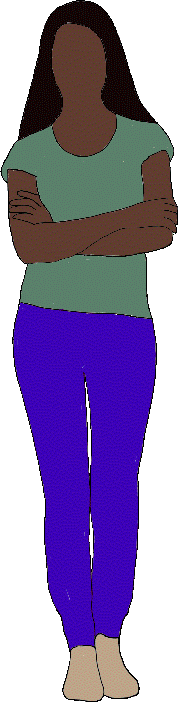
\includegraphics[width=0.04\textwidth]{figures/Relativity/woman_standing}};
}
{
\node[above=-0.5cm] at (-0.01*\L,0) {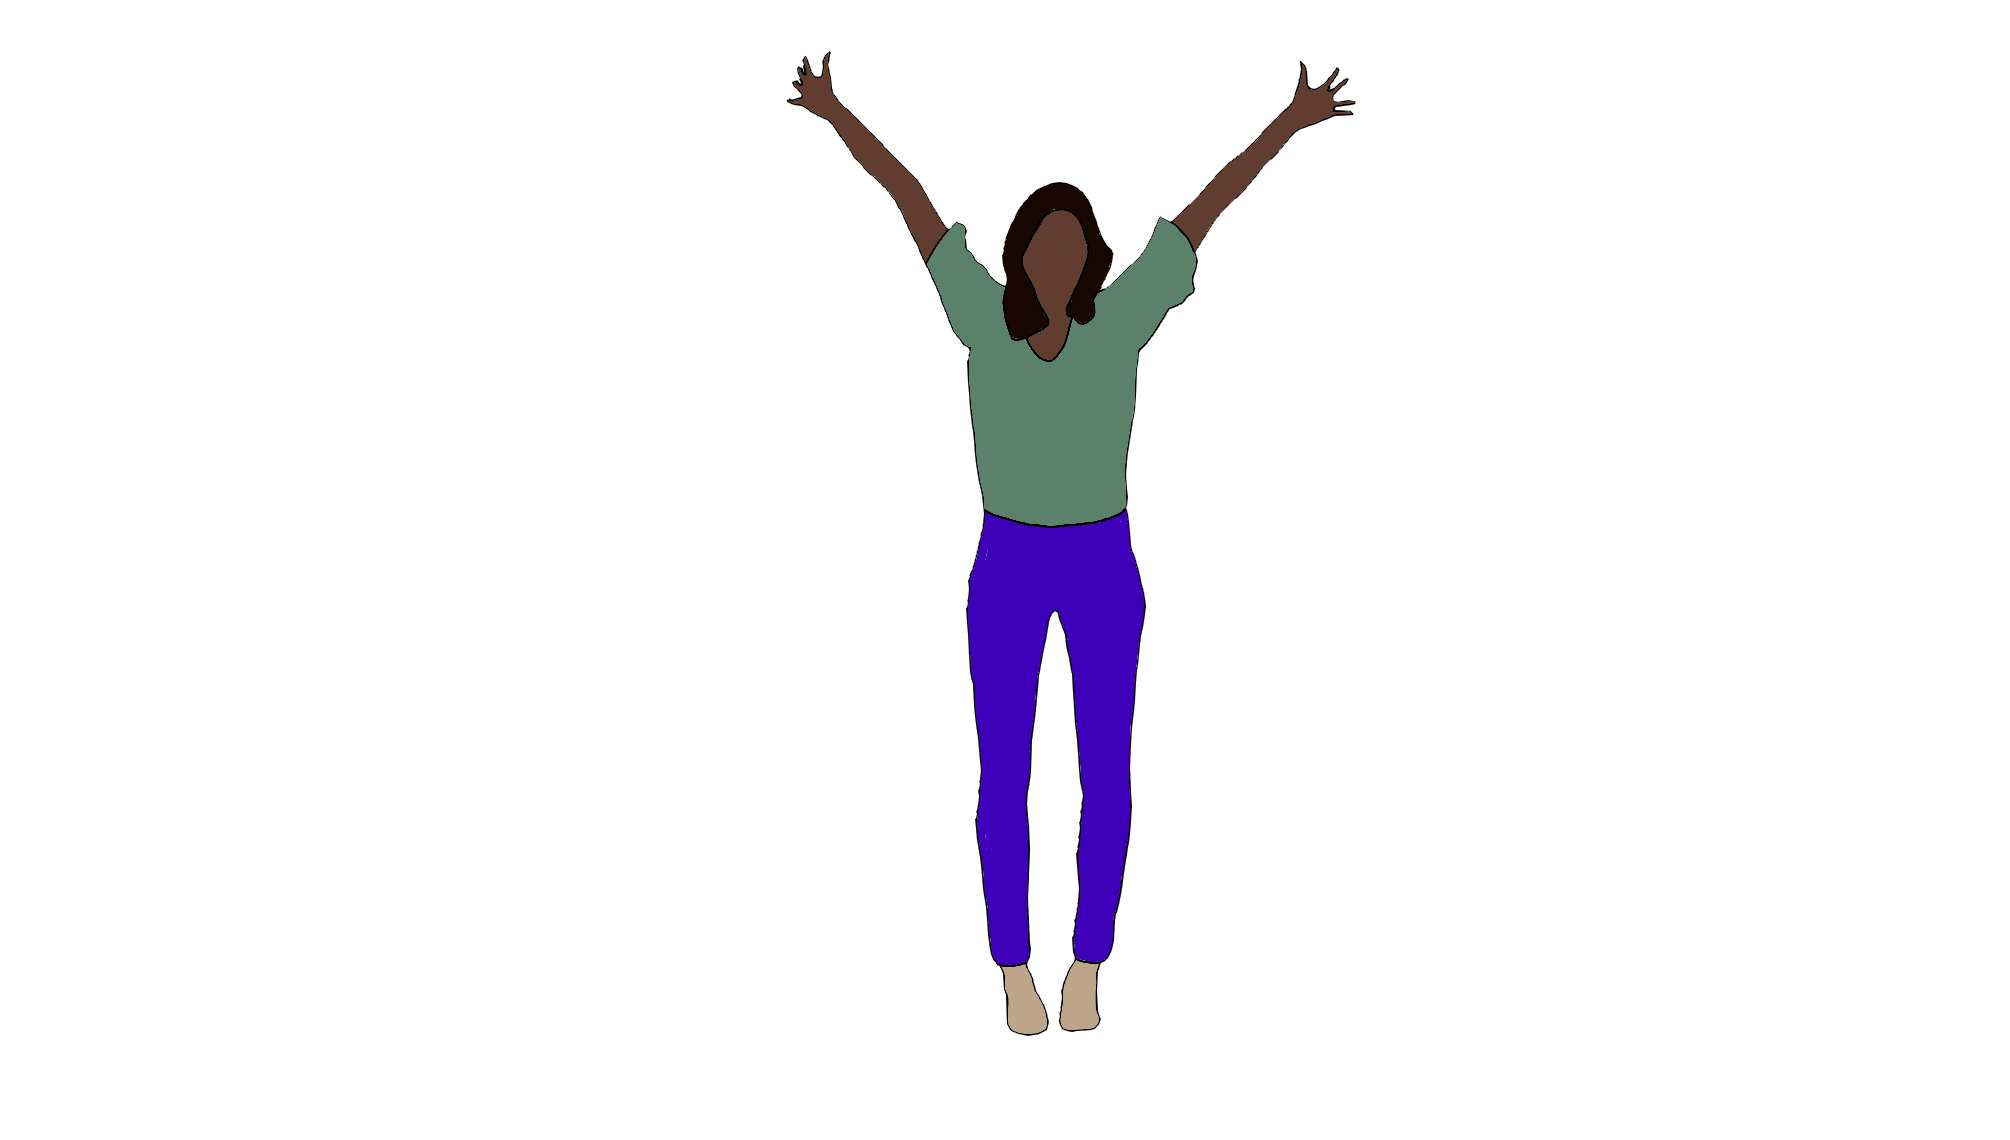
\includegraphics[width=0.4\textwidth]{figures/Relativity/alice_arms_png}};
}


\ifthenelse{\i<6}{
\node[above=-0.2cm] at (-0.4*\L,\h) {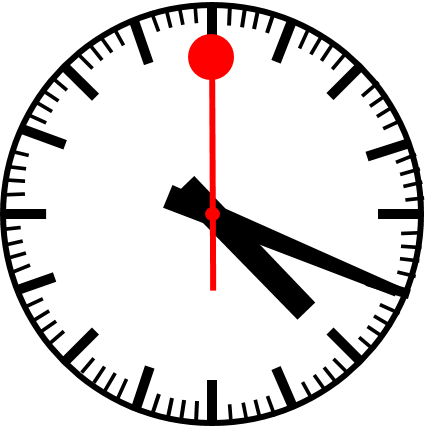
\includegraphics[width=0.07\textwidth]{figures/Relativity/fourtwenty.png}};
}{}
\ifthenelse{\i>5 \AND \i<12}{
\node[above=-0.2cm] at (-0.4*\L,\h) {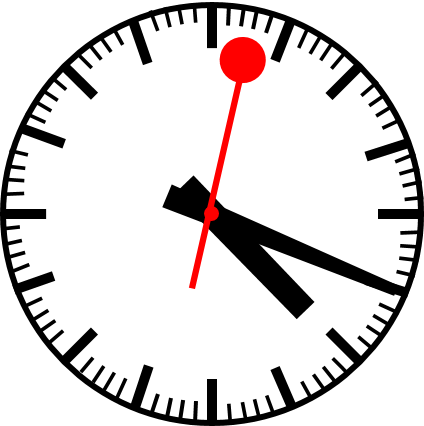
\includegraphics[width=0.07\textwidth]{figures/Relativity/fourtwenty_1.png}};
}{}
\ifthenelse{\i>11 \AND \i<18}{
\node[above=-0.2cm] at (-0.4*\L,\h) {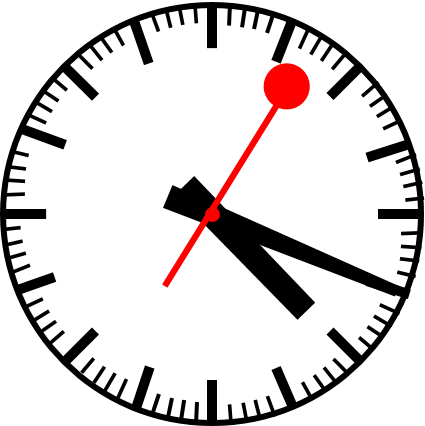
\includegraphics[width=0.07\textwidth]{figures/Relativity/fourtwenty_2.png}};
}{}
\ifthenelse{\i>17}{
\node[above=-0.2cm] at (-0.4*\L,\h) {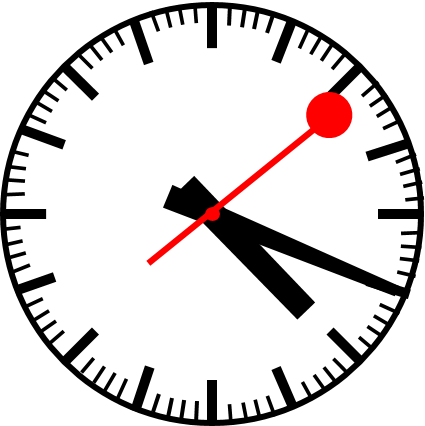
\includegraphics[width=0.07\textwidth]{figures/Relativity/fourtwenty_3.png}};
}{}

\ifthenelse{\i<6}{
\node[above=-0.2cm] at (0.4*\L,\h) {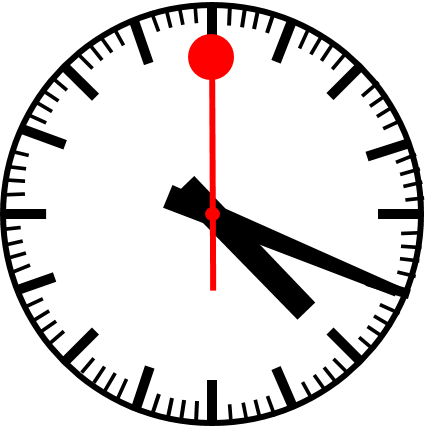
\includegraphics[width=0.07\textwidth]{figures/Relativity/fourtwenty.png}};
}{}
\ifthenelse{\i>5 \AND \i<12}{
\node[above=-0.2cm] at (0.4*\L,\h) {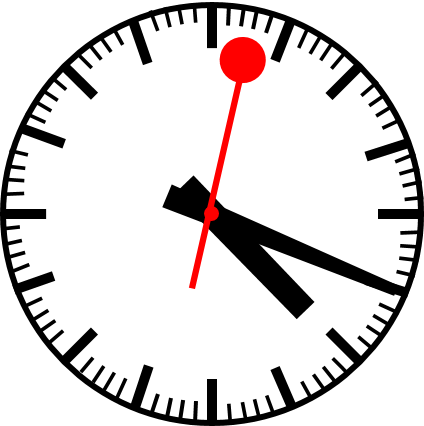
\includegraphics[width=0.07\textwidth]{figures/Relativity/fourtwenty_1.png}};
}{}
\ifthenelse{\i>11 \AND \i<18}{
\node[above=-0.2cm] at (0.4*\L,\h) {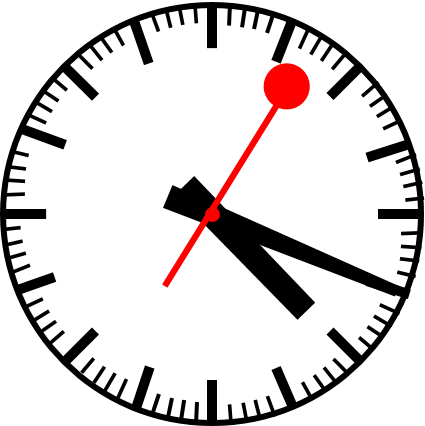
\includegraphics[width=0.07\textwidth]{figures/Relativity/fourtwenty_2.png}};
}{}
\ifthenelse{\i>17}{
\node[above=-0.2cm] at (0.4*\L,\h) {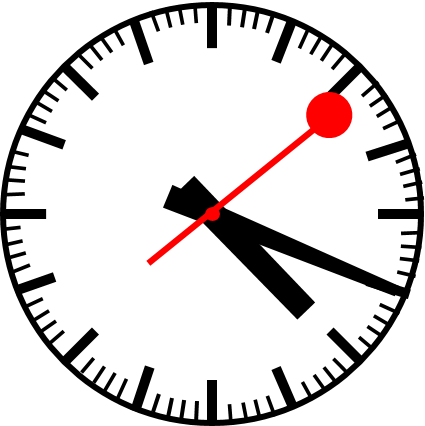
\includegraphics[width=0.07\textwidth]{figures/Relativity/fourtwenty_3.png}};
}{}

\end{tikzpicture}
}%multiframe
\end{animateinline}


\begin{itemize}
\item An observer on a platform is equidistant from 2 clocks that output pulses of light. When the clocks read 16:20, they output a light pulse, the observer sees the two light pulses at the same time and she concludes that the clock are synchronized.
\end{itemize}

\end{frame}



%% Simultaneity Animation 2
%%%%%%%%%%%%%%%%%%%%%%%%%%%%%%
\begin{frame}{Simultaneity}

\centering

\pgfmathtruncatemacro\N{24}
\begin{animateinline}[autoplay,loop]{4} % 5 fps, same as 0.2 s transduration

\multiframe{\N}{i=0+1}{

\tikzmath{
%\i=1;
\L=10;
\w=0.2;%thickness of platform
\h=2;
\D=0.3*\L;
\xs=0.25*\L-\i*0.5*\L/\N;%platform shift
\xr=\xs+0.33*\L-\i*\D/\N;%position of right laser
\xl=-\xs+0.33*\L+\i*\D/\N-1.12*\L;%position of left laser
}
\begin{tikzpicture}

\useasboundingbox (-0.7*\L,-\h) rectangle (0.7*\L,1.5*\h);


%moving platform
\begin{scope}[shift={(\xs,0)}]
%platform
\fill[color=black!70] (-\L/2,-\w) rectangle (\L/2,0);
%posts
\fill[color=qblue!70] (-0.42*\L,0) rectangle (-0.38*\L,0.97*\h);
\fill[color=qblue!70] (0.38*\L,0) rectangle (0.42*\L,0.97*\h);
\ifthenelse{\i<23}{
\node[above=-0.2cm] at (0,0) {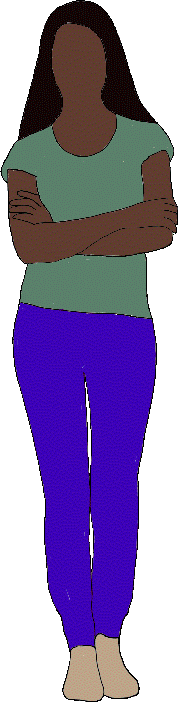
\includegraphics[width=0.04\textwidth]{figures/Relativity/woman_standing}};
}
{
\node[above=-0.5cm] at (-0.01*\L,0) {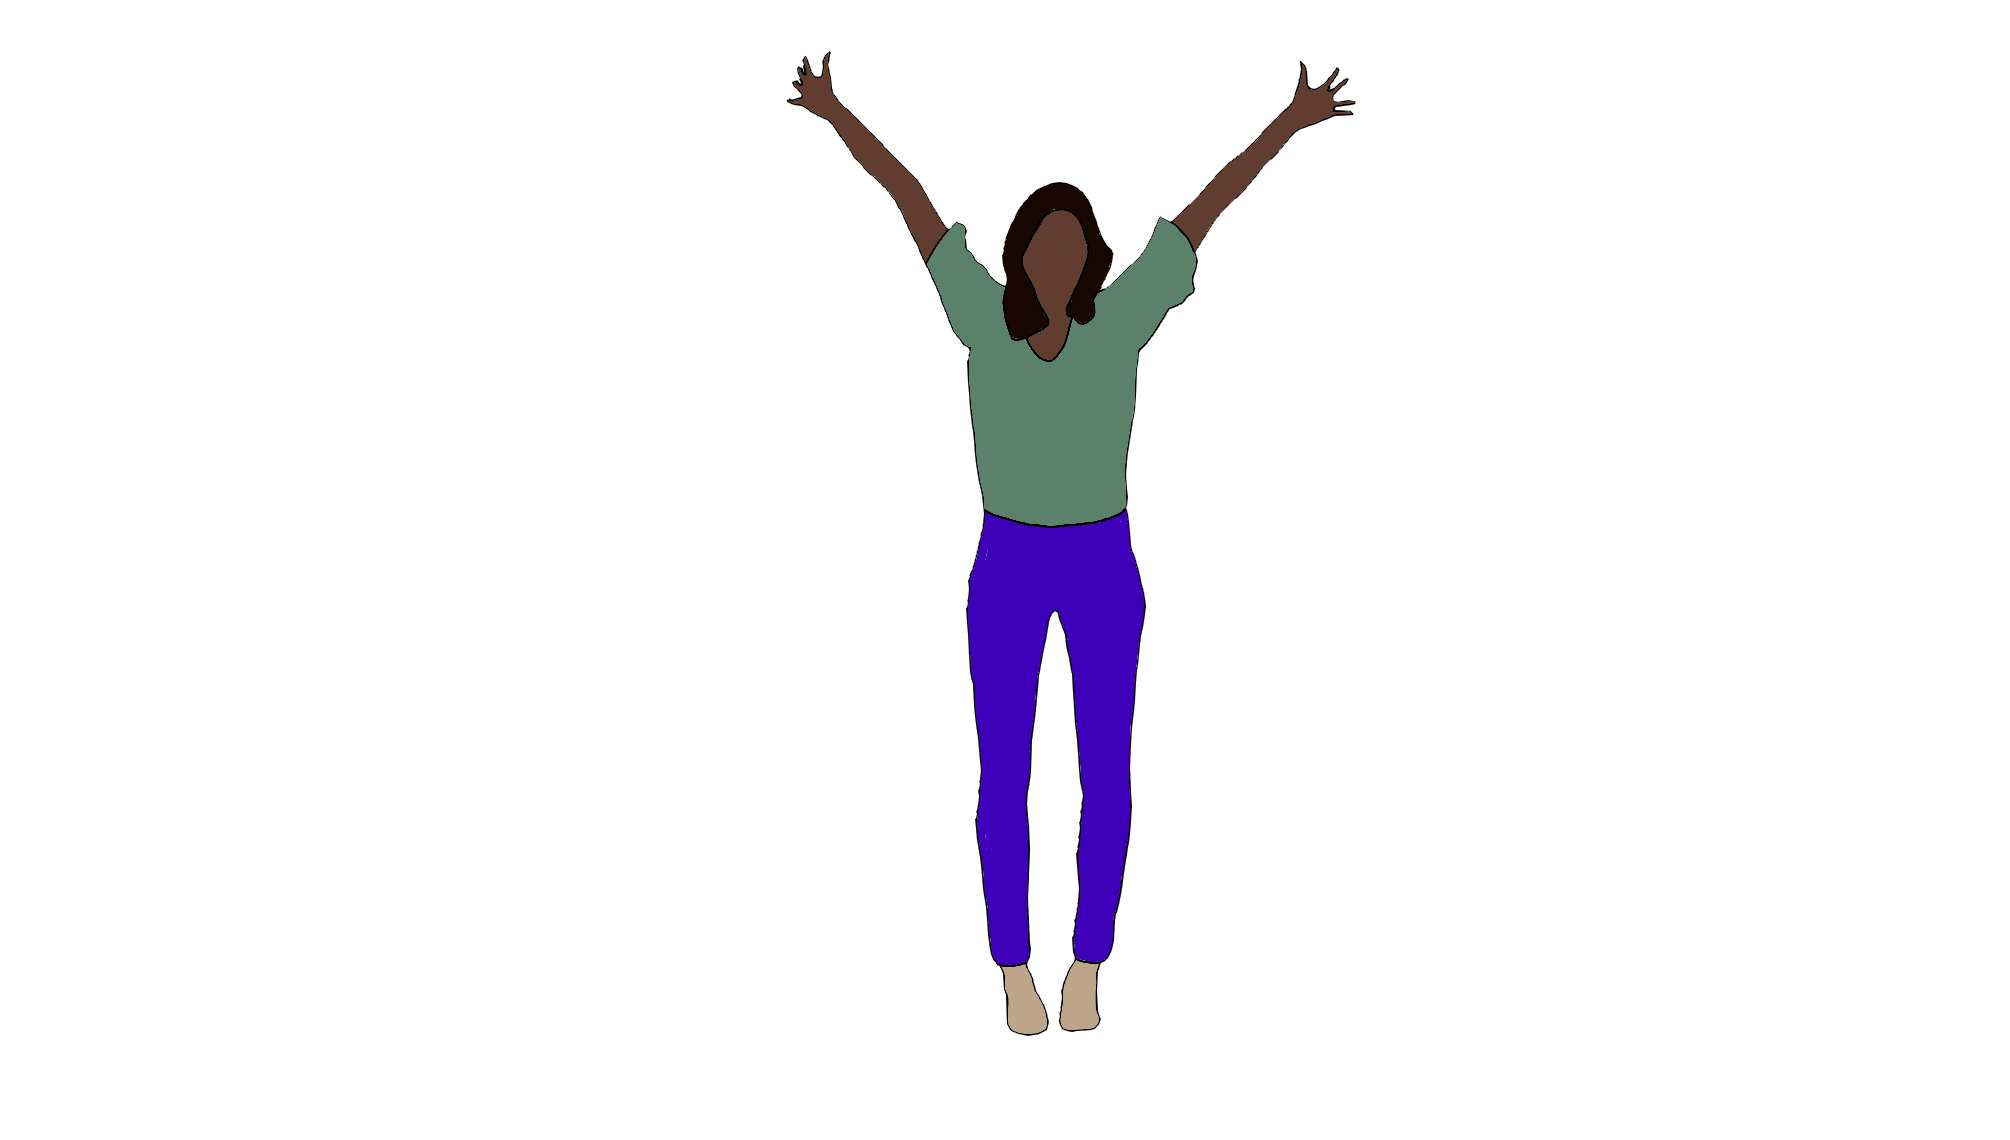
\includegraphics[width=0.4\textwidth]{figures/Relativity/alice_arms_png}};
}

%left clock
\ifthenelse{\i<5}{
\node[above=-0.2cm] at (-0.4*\L,\h) {
\includegraphics[width=0.07\textwidth]{figures/Relativity/fourtwenty_m3.png}};
}{}
\ifthenelse{\i>4 \AND \i<11}{
\node[above=-0.2cm] at (-0.4*\L,\h) {
\includegraphics[width=0.07\textwidth]{figures/Relativity/fourtwenty_m2.png}};
}{}
\ifthenelse{\i>10 \AND \i<17}{
\node[above=-0.2cm] at (-0.4*\L,\h) {
\includegraphics[width=0.07\textwidth]{figures/Relativity/fourtwenty_m1.png}};
}{}
\ifthenelse{\i>16}{
\node[above=-0.2cm] at (-0.4*\L,\h) {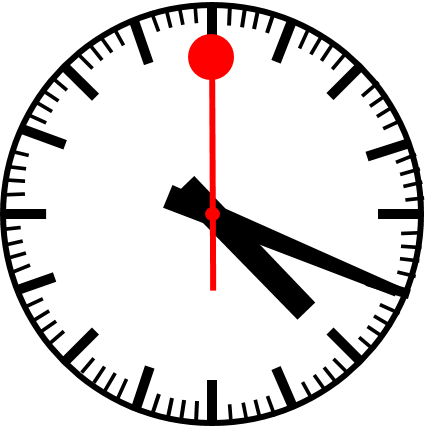
\includegraphics[width=0.07\textwidth]{figures/Relativity/fourtwenty.png}};
}{}


%right clock
\ifthenelse{\i<5}{
\node[above=-0.2cm] at (0.4*\L,\h) {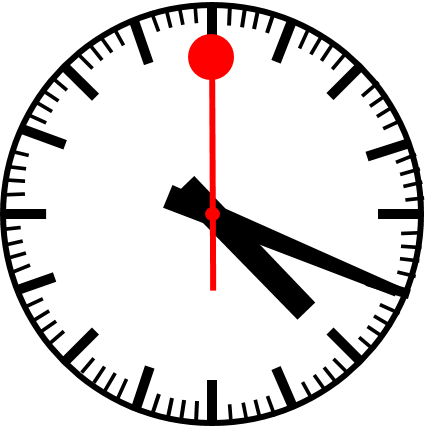
\includegraphics[width=0.07\textwidth]{figures/Relativity/fourtwenty.png}};
}{}
\ifthenelse{\i>4 \AND \i<11}{
\node[above=-0.2cm] at (0.4*\L,\h) {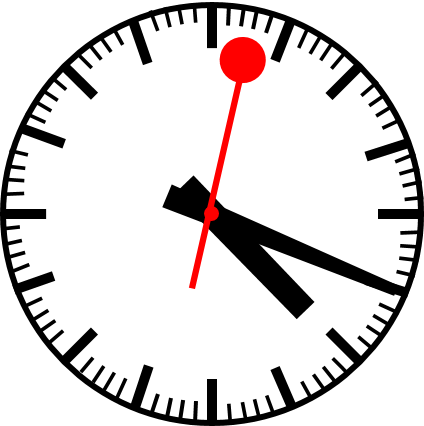
\includegraphics[width=0.07\textwidth]{figures/Relativity/fourtwenty_1.png}};
}{}
\ifthenelse{\i>10 \AND \i<17}{
\node[above=-0.2cm] at (0.4*\L,\h) {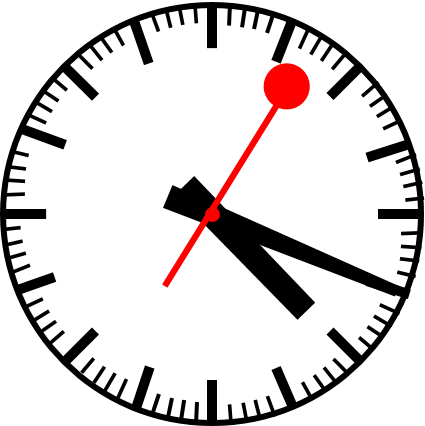
\includegraphics[width=0.07\textwidth]{figures/Relativity/fourtwenty_2.png}};
}{}
\ifthenelse{\i>16}{
\node[above=-0.2cm] at (0.4*\L,\h) {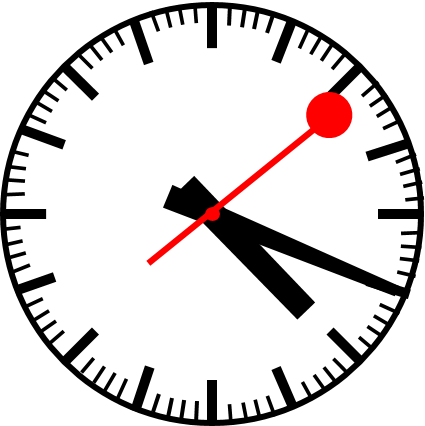
\includegraphics[width=0.07\textwidth]{figures/Relativity/fourtwenty_3.png}};
}{}

\end{scope}

%foreground person
\node[above=-0.5cm] at (-0.5*\L,-0.5*\h) {
\includegraphics[width=0.4\textwidth]{figures/Relativity/traincart}};
\node[above=0cm] at (-0.5*\L,-0.5*\h) {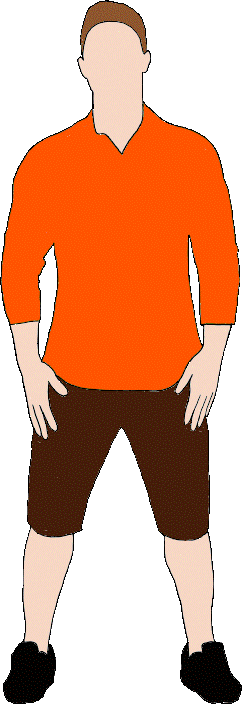
\includegraphics[width=0.06\textwidth]{figures/Relativity/man_standing_ink}};


%laser ball
\draw [color=qred, line width =1.5pt] (\xr,1.2*\h) -- (0.6*\L,1.2*\h);
\node [color=qred, star, star points=10, star point height=.1cm, minimum size=0.2cm, fill] at(\xr,1.2*\h) {};
\ifthenelse{\i>16}{
\draw [color=qred, line width =1.5pt] (\xl,1.2*\h) -- (-0.5*\L,1.2*\h);
\node [color=qred, star, star points=10, star point height=.1cm, minimum size=0.2cm, fill] at(\xl,1.2*\h) {};
}{}

\end{tikzpicture}
}%multiframe
\end{animateinline}

\begin{itemize}
\item An observer on a train sees the platform moving in his rest frame. He observes two pulses of light arrive at the same time at the person on the platform. 
\item He concludes that the pulse from the right happened first, since the pulses travel at speed $c$ and the one from the right travelled further. He disagrees that the clocks are synchronized! \textbf{But, causality...}
\end{itemize}

\end{frame}



%%%%%%%%%%%%%%%%%%%%%%%%%%%%%%
\begin{bulletframe}{Defining ``events'' and frames of reference}
\item We considered the ``event'': \emph{``The person on the platform received two pulses of light at the same time.''}
\item We did not consider the ``event'': \emph{``The two clocks emitted a pulse of light at the same time.''}
\item This led to the conclusion that simultaneity is relative:
\begin{itemize}
\item The second statement is not an ``event'' because the two clocks are at different positions in space. 
\item[$\rightarrow$] We can only compare things that happen at the same location in space and time. An ``event'' is something that occurs at a single location in space and time.
\item[$\rightarrow$] We introduce ``space-time'', and we say that an event is something that happens in four-dimensional space-time and has coordinates (x,y,z,t)
\item[$\rightarrow$] We can then compare if events in space-time are simultaneous or not:
\begin{itemize}
\item[$\rightarrow$] ''Person receiving two pulses of light'' is always after ``clock A'' and  ``clock B'' emit a pulse of light. You can check this out; the only way for this not to be true is if one of the observers goes faster than c.
\item[$\rightarrow$] ``clock A emits a pulse of light'' is not always at the same time as ``clock B emits a pulse of light''. We just showed that it can be before or after as well!
\end{itemize}
\end{itemize}

\end{bulletframe}


%%%%%%%%%%%%%%%%%%%%%%%%%%%%%%



%%%%%%%%%%%%%%%%%%%%%%%%%%%%%%
\subsection{Example question}
\label{subsec:examplequestion}
\twocolframesf{Example question}
{
\begin{itemize}
\item Repulsive force per unit length between two charged wires:
\begin{align*}
\frac{F^E_0}{l}=\frac{\lambda_0}{2\pi \epsilon_0 r}
\end{align*}
\item Attractive force per unit length between two current carrying wires:
\begin{align*}
\frac{F^B_0}{l}=\frac{\mu_0 I^2}{2\pi r}
\end{align*}
\end{itemize}
}
{
\centering
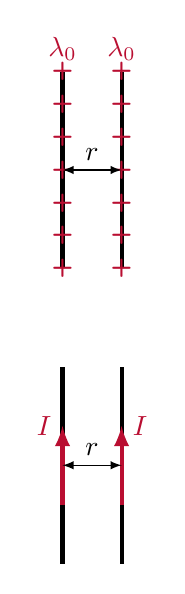
\begin{tikzpicture}
\tikzmath{
\r=0.75;
\L=2.5;
\Np=6;
}
%top part:
%\wires
\draw[line width=1.5] (-\r/2,-\L/2) -- (-\r/2,\L/2) node[above,color=qred] {$\lambda_0$};
\draw[line width=1.5] (\r/2,-\L/2) -- (\r/2,\L/2) node[above,color=qred] {$\lambda_0$};
%charges
\foreach \i in {0,...,\Np}{
 \tikzmath{
   \yp=-\L/2+\i*\L/\Np;
 }
 \node[color=qred] at (-\r/2,\yp) {\small \textbf{+}};
 \node[color=qred] at (\r/2,\yp) {\small \textbf{+}};
}
%labels
\draw[latex-latex] (-\r/2,0) -- (\r/2,0) node[midway,above]{$r$};

\begin{scope}[shift={(0,-1.5*\L)}]
%\wires
\draw[line width=1.5] (-\r/2,-\L/2) -- (-\r/2,\L/2) ;
\draw[line width=1.5] (\r/2,-\L/2) -- (\r/2,\L/2) ;
%current
\draw[line width=1.5, color=qred,-latex] (-\r/2,-0.2*\L) -- (-\r/2,0.2*\L) node[left]{$I$};
\draw[line width=1.5, color=qred,-latex] (\r/2,-0.2*\L) -- (\r/2,0.2*\L) node[right]{$I$};
%labels
\draw[latex-latex] (-\r/2,0) -- (\r/2,0) node[midway,above]{$r$};
\end{scope}
\end{tikzpicture}

}

%%%%%%%%%%%%%%%%%%%%%%%%%%%%%%
\twocolframesf{Example question}
{
\only<1>{
\begin{itemize}
\item In a frame moving downwards with speed $v$, it looks like there is an upwards current given by:
\begin{align*}
I=\frac{dQ}{dt}=\frac{d(\lambda l)}{dt}=\lambda v
\end{align*}
\item \textbf{Let us assume that the laws of physics and that the constants of nature remain the same in this frame of reference}. The force on one of the wires must remain the same:
\begin{align*}
\frac{F^E_0}{l}=\frac{\textcolor{qred}{\lambda_0}}{2\pi \epsilon_0 r}=\frac{\textcolor{qred}{\lambda}}{2\pi \epsilon_0 r}-\frac{\mu_0 I^2}{2\pi r}
\end{align*}
\end{itemize}
Charge density is the only thing that can be different in the moving frame, so we call it $\textcolor{qred}{\lambda}$. 
}
\only<2>{
Working through the math:
\begin{align*}
\frac{\lambda_0}{2\pi \epsilon_0 r}&=\frac{\lambda}{2\pi \epsilon_0 r}-\frac{\mu_0 (\lambda v)^2}{2\pi r}\\
\frac{\lambda_0}{\epsilon_0 r}&=\frac{\lambda}{\epsilon_0}-\mu_0 (\lambda v)^2\\
\lambda_0^2&=\lambda^2(1-\epsilon_0\mu_0v^2)\\
\therefore \lambda &= \lambda_0 \frac{1}{\sqrt{1-\epsilon_0\mu_0v^2}}\\
\Aboxed{\therefore \lambda &=\lambda_0 \frac{1}{\sqrt{1-\frac{v^2}{c^2}}}}
\end{align*}
From Maxwell's equations: $c=\frac{1}{\sqrt{\epsilon_0\mu_0}}$
}
\only<3>{
The charge density \emph{is} different in the moving frame of reference (and larger since $v < c$):
\begin{align*}
\lambda &=\lambda_0 \frac{1}{\sqrt{1-\frac{v^2}{c^2}}}
\end{align*}
\begin{itemize}
\item Observers in the two reference frames can agree on the number of charges in a section of wire (they could literally count the charges between 2 lines drawn on the wire). 
\item The only way for the charge density to be higher in the moving reference frame is if \textbf{the wire is actually shorter (the lines are closer)!}
\end{itemize}
}
}
{
\centering
\pgfmathtruncatemacro\N{10}
\begin{animateinline}[autoplay,loop]{4} % 5 fps, same as 0.2 s transduration
\multiframe{\N}{i=0+1}{

\begin{tikzpicture}
\tikzmath{
\r=0.75;
\L=5.;
\Np=12;
\Npp=12;
\dy=\i*\L/\Npp/\N;
}
\only<3>{
\tikzmath{
\Npp=18;
\dy=\i*\L/\Npp/\N;
}
}

%first wire pair
%\wires
\draw[line width=1.5] (-\r/2,-\L/2) -- (-\r/2,\L/2) node[above,color=qred] {$\lambda_0$};
\draw[line width=1.5] (\r/2,-\L/2) -- (\r/2,\L/2) node[above,color=qred] {$\lambda_0$};
%charges
\foreach \iy in {0,...,\Np}{
 \tikzmath{
   \yp=-\L/2+\iy*\L/\Np;
 }
 \node[color=qred] at (-\r/2,\yp) {\small \textbf{+}};
 \node[color=qred] at (\r/2,\yp) {\small \textbf{+}};
}
%labels
\draw[latex-latex] (-\r/2,0) -- (\r/2,0) node[midway,above]{$r$};
\only<3>{
\draw[line width=2, color=qblue!70] (-0.6*\r,0.25*\L) -- (0.6*\r,0.25*\L);
\draw[line width=2, color=qblue!70] (-0.6*\r,-0.25*\L) -- (0.6*\r,-0.25*\L);
}


%second wire
\begin{scope}[shift={(3*\r,0)}]
%\wires
\draw[line width=1.5] (-\r/2,-\L/2) -- (-\r/2,\L/2) node[above,color=qred] {$\lambda$};
\draw[line width=1.5] (\r/2,-\L/2) -- (\r/2,\L/2) node[above,color=qred] {$\lambda$};
%charges
\foreach \iy in {1,...,\Npp}{
 \tikzmath{
   \yp=-\L/2+(\iy-1)*\L/\Npp+\dy;
 }
 \node[color=qred] at (-\r/2,\yp) {\small \textbf{+}};
 \node[color=qred] at (\r/2,\yp) {\small \textbf{+}};
 }
%current
\draw[line width=1.5, color=qred,-latex] (-0.8*\r,-0.2*\L) -- (-0.8*\r,0.2*\L) node[left]{$I$};
\draw[line width=1.5, color=qred,-latex] (0.8*\r,-0.2*\L) -- (0.8*\r,0.2*\L) node[right]{$I$};
\only<3>{
\draw[line width=2, color=qblue!70] (-0.6*\r,0.25*\L*\Np/\Npp) -- (0.6*\r,0.25*\L*\Np/\Npp);
\draw[line width=2, color=qblue!70] (-0.6*\r,-0.25*\L*\Np/\Npp) -- (0.6*\r,-0.25*\L*\Np/\Npp);
}
%labels
\draw[latex-latex] (-\r/2,0) -- (\r/2,0) node[midway,above]{$r$};
\end{scope}
\end{tikzpicture}
}%multiframe
\end{animateinline}
\captionof*{figure}{\textit{Two charged wires viewed at rest (left) and from a frame of reference that is moving downwards (right).}}
}


%%%%%%%%%%%%%%%%%%%%%%%%%%%%%%
\subsection{Length contraction}
\label{subsec:lengthcontraction}
\twocolframesf{Length contraction}
{
\begin{itemize}
\item An object that is moving is shorter in the direction of motion than you would measure if the object were at rest.
\item This is real, stuff shrinks lengthwise as it moves fast.
\begin{align*}
L=L_0\sqrt{1-\frac{v^2}{c^2}}<L_0
\end{align*}
\end{itemize}
}
{
\centering
\begin{tikzpicture}
\begin{scope}
\clip(-2,-2) rectangle (2.2,2);
\node at (0,-1) {
\includegraphics[width=0.8\textwidth, height=0.3\textwidth]{figures/Relativity/qtrain}};
\node at (0,1) {
\includegraphics[width=1\textwidth, height=0.3\textwidth]{figures/Relativity/qtrain}};
\end{scope}

\draw[latex-latex] (-1.6,2) -- (1.9,2)node[midway,above]{$L_0$};
\draw[latex-latex] (-1.2,-1.8) -- (1.7,-1.8)node[midway,below]{$L$};

\end{tikzpicture}
}

%%%%%%%%%%%%%%%%%%%%%%%%%%%%%%
%%%%%%%%%%%%%%%%%5should animate (doesn work?)
%%%%%%%%%%%%%%%%%%%%%%%%%%%%%%
\subsection{Special relativity and E/M}
\label{subsec:speacialrelativityandem}
\twocolframesf{Special Relativity and E/M}
{
\begin{itemize}
\item A (neutral) wire carries current (electrons moving to the right relative to stationary ions).
\item We place a charge $+Q$ near the wire, it feels no net force. 
\item We would say the current creates a magnetic field out of the page, but since $Q$ is not moving, it feels no force ($\vec F=Q \vec v \times \vec B$).
\item<2> If $Q$ moved towards the right, it would feel a downward magnetic force.
\end{itemize}
}
{
\centering
\pgfmathtruncatemacro\N{10}
\begin{animateinline}[autoplay,loop]{4} % 5 fps, same as 0.2 s transduration
\multiframe{\N}{i=0+1}{
\begin{tikzpicture}
\tikzmath{
\L=4.5;
\r=1.2;
\h=1.5*\r;
\Np=10;
\Ne=10;
\dy=\i*\L/\Ne/\N;
}
%\useasboundingbox (-0.7*\L,-2*\r) rectangle (0.7*\L,1.2*\r);
\draw[opacity=0] (-0.7*\L,-3*\r) rectangle (0.6*\L,1.2*\r);
%wire
\fill[color=black!70,opacity=0.8] (-\L/2,-\r/2) rectangle (\L/2,\r/2) ;
%electrons and ions
\foreach \ip in {1,...,\Np}{
  \tikzmath{
   \xp=-\L/2+\ip*\L/\Np-0.5*\L/\Np;
  }
 \fill[color=qblue] (\xp,0.2*\r) circle (5pt);
 \node[color=white] at (\xp,0.2*\r) {+};
}
\begin{scope}%cut the charges exiting the edge...
\clip (-\L/2,-\r/2) rectangle (\L/2,\r/2) ;
\foreach \ip in {1,...,\Ne}{
  \tikzmath{
   \xe=-\L/2+(\ip-1)*\L/\Ne+\dy;
  }
 \fill[color=qred] (\xe,-0.2*\r) circle (3pt);
 \node[text=white] at (\xe,-0.2*\r) {-};
}
\end{scope}
%charge
\fill[color=qblue] (0,-\h) circle (3pt);
\node[left,color=qblue] at (0,-\h) {$+Q$};
\only<2>{
\draw[-latex, line width=1.5] (0,-\h) -- +(1,0) node[right]{$\vec v$};
\draw[-latex, line width=1.5] (0,-\h) -- +(0,-1) node[left]{$\vec F_B$};
}


%Labels
\node[left,color=qblue] at (-0.2*\L,-\h) {$\vec B\;\odot$};
\draw[-latex, line width=1.5] (0.1*\L,0.75*\r) -- (-0.1*\L,0.75*\r) node[midway,above]{$I$};
\draw[latex-, line width=1.5, color=qred] (0.1*\L,-0.75*\r) -- (-0.1*\L,-0.75*\r) node[midway,below]{$\vec v_d$};

\end{tikzpicture}
}%multiframe
\end{animateinline}
\captionof*{figure}{\textit{In the reference frame of the wire: A charge is near a wire with current. The charge feels a magnetic force if it moves relative to the wire.}}
}

%%%%%%%%%%%%%%%%%%%%%%%%%%%%%%
%%%%%%%%%shoujld animate as well, also doesn't  work
%%%%%%%%%%%%%%%%%%%%%%%%%%%%%%
\twocolframesf{Special Relativity and E/M}
{
Suppose that $Q$ moves to the right, \emph{with the same speed as the electrons}. \textbf{In the frame of $Q$}:
\begin{itemize}
\item<2-> The electrons are immobile and \emph{are sparse} (they were length contracted).
\item<2-> The ions move to the left and \emph{are denser} (they are length contracted).
\item<3->[$\rightarrow$] The wire no longer appears neutral and repels $Q$ by the \textbf{electric force}, which must have the same magnitude.
\item<3->[$\rightarrow$] Since $Q$ is stationary, there is no force from the magnetic field due to the moving ions.
\item<3->[$\rightarrow$] The magnetic and electric force are really different aspects of the same effect, Special Relativity is the connection!
\end{itemize}
}
{
\centering
\pgfmathtruncatemacro\N{10}
\begin{animateinline}[autoplay,loop]{4} % 5 fps, same as 0.2 s transduration
\multiframe{\N}{i=0+1}{
\begin{tikzpicture}
\tikzmath{
\L=4.5;
\r=1.2;
\h=1.5*\r;
\Np=12;
\Ne=7;
\dy=\i*\L/\Np/\N;
}
%\useasboundingbox (-0.7*\L,-2*\r) rectangle (0.7*\L,1.2*\r);
\draw[opacity=0] (-0.7*\L,-3*\r) rectangle (0.6*\L,1.2*\r);
%wire
\fill[color=black!70,opacity=0.8] (-\L/2,-\r/2) rectangle (\L/2,\r/2) ;
%electrons and ions
\begin{scope}%cut the charges exiting the edge...
\clip (-\L/2,-\r/2) rectangle (\L/2,\r/2) ;
\foreach \ip in {1,...,\Np}{
  \tikzmath{
   \xp=-\L/2+(\ip)*\L/\Np-\dy;
  }
 \fill[color=qblue] (\xp,0.2*\r) circle (5pt);
 \node[color=white] at (\xp,0.2*\r) {+};
}
\end{scope}
\foreach \ip in {1,...,\Ne}{
  \tikzmath{
   \xe=-\L/2+\ip*\L/\Ne-0.5*\L/\Ne;
  }
 \fill[color=qred] (\xe,-0.2*\r) circle (3pt);
 \node[text=white] at (\xe,-0.2*\r) {-};
}

%charge
\fill[color=qblue] (0,-\h) circle (3pt);
\node[left,color=qblue] at (0,-\h) {$+Q$};
\only<3->{
\draw[-latex, line width=1.5] (0,-\h) -- +(0,-1) node[left]{$\vec F_E$};
}
%Labels
\node[left,color=qblue] at (-0.2*\L,-\h) {$\vec B'\;\odot$};
\draw[-latex, line width=1.5] (0.1*\L,0.75*\r) -- (-0.1*\L,0.75*\r) node[midway,above]{$I'$};

\end{tikzpicture}
}%multiframe
\end{animateinline}
\only<1-2>{
\captionof*{figure}{\textit{In the reference frame of the charge moving with the electrons.}}
}
\only<3>{
\captionof*{figure}{\textit{In the reference frame of the charge moving with the electrons. It feels a purely electric force due to the apparent net charge on the wire.}}
}
}

%%%%%%%%%%%%%%%%%%%%%%%%%%%%%%
\subsection{Einstein's Clock}
\label{subsec:einsteinsclock}
\twocolframesf{Einstein's Clock}
{
\begin{itemize}
\item A beam of light bounces back and forth between 2 mirrors.
\item You watch the light beam, and determine that the time for a return trip of the light is:
\begin{align*}
\Delta \tau = \frac{2D}{c}
\end{align*}
\end{itemize}
The speed of light is:
\begin{align*}
c= \frac{2D}{\tau}
\end{align*}
Note: You measure the time difference between two events at the same position, as far as you are concerned.
}
{
\centering
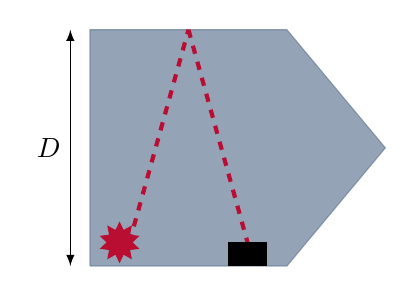
\begin{tikzpicture}
\tikzmath{
\D=3;
\L=5;
}
\fill[draw=black,color=qblue!60,opacity=0.7] (0,-\D/2) -- (0,\D/2) -- (\L/2,\D/2) -- (0.75*\L,0) --  (\L/2,-\D/2) -- (0,-\D/2);

\node [color=qred, star, star points=10, star point height=.1cm, minimum size=0.2cm, fill] at (0.075*\L,-0.4*\D) {};
\draw[color=qred,line width=1.5,dashed] (0.1*\L,-0.4*\D) -- (0.25*\L,0.5*\D); 
\draw[color=qred,line width=1.5,dashed]  (0.25*\L,0.5*\D) -- (0.4*\L,-0.4*\D); 
\fill (0.35*\L,-0.5*\D) rectangle (0.45*\L,-0.4*\D);
\draw[latex-latex] (-0.05*\L,-\D/2) -- (-0.05*\L,\D/2) node[midway, left] {$D$};

\end{tikzpicture}
\captionof*{figure}{\textit{A beam of light can be used as a clock in this spaceship. Here the path of the beam is viewed in the reference frame of the spaceship.}}
}



%%%%%%%%%%%%%%%%%%%%%%%%%%%%%%
\twocolframesf{Einstein's Clock}
{
\begin{itemize}
\item You take your clock on a spaceship and someone on Earth observes the light beam.
\item The light travels a longer distance as far as they are concerned, but the speed of the light beam is still $c$ (in the diagonal direction in the above diagram).
\item They measure the time difference between events that happen at different locations.
\item They would write the speed of light as:
\begin{align*}
c= \frac{2\sqrt{D^2+l^2}}{\Delta t}=\frac{2\sqrt{D^2+\left(\frac{v\Delta t}{2} \right)^2}}{\Delta t}
\end{align*}
\end{itemize}
}
{
\centering
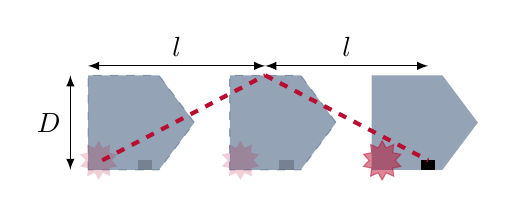
\begin{tikzpicture}
\tikzmath{
\D=3;
\L=4.5;
\fss=0.4;
}
\begin{scope}[shift={(-0.4*\L,0)}, scale=\fss, opacity=0.2]
\fill[draw=black, dashed,color=qblue!60,opacity=0.7] (0,-\D/2) -- (0,\D/2) -- (\L/2,\D/2) -- (0.75*\L,0) --  (\L/2,-\D/2) -- (0,-\D/2);
\node [color=qred, star, star points=10, fill] at (0.075*\L,-0.4*\D) {};
\fill (0.35*\L,-0.5*\D) rectangle (0.45*\L,-0.4*\D);
\end{scope}

\begin{scope}[shift={(0,0)}, scale=\fss, opacity=0.2]
\fill[draw=black, dashed, color=qblue!60,opacity=0.7] (0,-\D/2) -- (0,\D/2) -- (\L/2,\D/2) -- (0.75*\L,0) --  (\L/2,-\D/2) -- (0,-\D/2);
\node [color=qred, star, star points=10, fill] at (0.075*\L,-0.4*\D) {};
\fill (0.35*\L,-0.5*\D) rectangle (0.45*\L,-0.4*\D);
\end{scope}

\begin{scope}[shift={(0.4*\L,0)}, scale=\fss]
\fill[color=qblue!60,opacity=0.7] (0,-\D/2) -- (0,\D/2) -- (\L/2,\D/2) -- (0.75*\L,0) --  (\L/2,-\D/2) -- (0,-\D/2);
\node [draw=black,color=qred, star, star points=10, fill, opacity=0.5] at (0.075*\L,-0.4*\D) {};
\fill (0.35*\L,-0.5*\D) rectangle (0.45*\L,-0.4*\D);
\end{scope}

%light ray
\draw[color=qred,line width=1.5,dashed] (-0.4*\L+\fss *0.1*\L,-\fss*0.4*\D) -- (\fss*0.25*\L,\fss*0.5*\D); 
\draw[color=qred,line width=1.5,dashed]  (\fss*0.25*\L,\fss*0.5*\D) -- (0.4*\L+\fss*0.4*\L,-\fss*0.4*\D); 
%labels
\draw[latex-latex] (-0.45*\L,-\fss*\D/2) -- (-0.45*\L,\fss*\D/2) node[midway, left] {$D$};
\draw[latex-latex] (-0.4*\L,\fss*1.2*\D/2) -- (\fss*0.25*\L,\fss*1.2*\D/2) node[midway, above] {$l$};
\draw[latex-latex] (\fss*0.25*\L,\fss*1.2*\D/2) -- (0.4*\L+\fss*0.4*\L,\fss*1.2*\D/2) node[midway, above] {$l$};

\end{tikzpicture}
\captionof*{figure}{\textit{A beam of light can be used as a clock in this spaceship. Here, the path of the beam is viewed by someone on Earth, as the spaceship moves to the right with speed, $v$.}}
\only<2>{
Re-arranging to isolate time, $\Delta t$:
\begin{align*}
\Delta t = \frac{2D}{c\sqrt{1-\frac{v^2}{c^2}}}=\frac{\Delta \tau}{\sqrt{1-\frac{v^2}{c^2}}}
\end{align*}
}
}

%%%%%%%%%%%%%%%%%%%%%%%%%%%%%%
\subsection{The gamma factor}
\label{subsec:thegammafactor}
\begin{frame}{Gamma}
\begin{itemize}
\item The factor:
\begin{align*}
\gamma = \frac{1}{\sqrt{1-\frac{v^2}{c^2}}}
\end{align*}
\end{itemize}
comes up a lot, so we call it $\gamma$. $v$ is the relative speed between two observers in inertial frames of reference. 
\end{frame}


%%%%%%%%%%%%%%%%%%%%%%%%%%%%%%



%%%%%%%%%%%%%%%%%%%%%%%%%%%%%%
\subsection{Time dilation}
\label{subsec:timedilation}
\begin{frame}{Time dilation}
\begin{align*}
\Delta t = \gamma \Delta \tau = \frac{1}{\sqrt{1-\frac{v^2}{c^2}}} \Delta\tau
\end{align*}
\begin{itemize}
\item The \textbf{``proper time''}, $\Delta\tau$, is the time that someone measures in their own reference frame (e.g. moving with the clock).
\item $\Delta t$ is the time that would be measured in a frame that is moving with speed $v$ relative to the frame were $\Delta\tau$ is measured.
\item Because $\gamma>1$ ,\textbf{ $\Delta t> \Delta \tau$ $\rightarrow$ ``Time dilation''}.
\item[$\rightarrow$] The time measured in the moving reference frame is always longer than the proper time that is measured in a stationary frame.
\item[$\rightarrow$]  This is not a thought experiment, time actually goes by slower, it's experimentally verified. 
\end{itemize}

\end{frame}




%%%%%%%%%%%%%%%%%%%%%%%%%%%%%%
\subsection{Muons}
\label{subsec:muons}
\twocolframesf{Muons}
{
\begin{itemize}
\item Muons are particles that radioactively decay in \SI{2.2}{\mu s} (\SI{2.2e-6}{s}).
\item They are produced when cosmic rays hit our atmosphere, at about 10km of altitude.
\item If they travel at essentially the speed of light, then to reach the Earth’s surface, it takes them:
\begin{align*}
t=\frac{d}{v}\sim\frac{\SI{10}{km}}{c}=\SI{3e-5}{s}
\end{align*}
$\rightarrow$ ~10x times their lifetime, so we should see very few muons at the Earth’s surface… but we see plenty (about 100,000 more than we’d expect!).
\end{itemize}
}
{
\capfig{1.0}{figures/Relativity/muons}{Illustration of cosmic rays generating muons in the atmosphere. \tiny\url{http://twinparadox.net/}}
}



%%%%%%%%%%%%%%%%%%%


\subsection{Time dilation implies length contraction}
\label{subsec:timedilationimplieslengthcontraction}
\begin{frame}{Time dilation \emph{implies} length contraction}
\begin{itemize}
\item Since you saw the Earth move away at speed $\sim c$ for about 4.5 years before you got to the star, you conclude that the star is about 4.5 light years from Earth.
\item You experience length contraction:
\begin{align*}
L=\frac{L_0}{\gamma}
\end{align*}
\item[$\rightarrow$] The proper length, $L_0$, is the length as measured in a frame at rest with respect to the object.
\end{itemize}
If you are at rest with the Earth and star, you measure that they are $L_0=100$ light years apart. If you move with respect to them, you measure a shorter distance, $L$. 
\end{frame}



%%%%%%%%%%%%%%%%%%%%%%%%%%%%%%



%%%%%%%%%%%%%%%%%%%%%%%%%%%%%%
\subsection{Relativistic train}
\twocolframesf{Relativistic train}
{
\begin{itemize}
\item You are moving with the train, so you measure the proper length of the train at rest.
\item People on Earth see the train moving, so they see it being contracted.
\begin{align*}
L=L_0\sqrt{1-\frac{v^2}{c^2}}<L_0
\end{align*}
\end{itemize}
}
{
\centering
\begin{tikzpicture}
\begin{scope}
\clip(-2,-2) rectangle (2.2,2);
\node at (0,-1) {
\includegraphics[width=0.8\textwidth, height=0.3\textwidth]{figures/Relativity/qtrain}};
\node at (0,1) {
\includegraphics[width=1\textwidth, height=0.3\textwidth]{figures/Relativity/qtrain}};
\end{scope}
\draw[-latex,line width=2pt,color=qred] (1.7,-0.8) -- +(1,0) node[midway,above]{$\vec v$};

\draw[latex-latex] (-1.6,2) -- (1.9,2)node[midway,above]{$L_0$};
\draw[latex-latex] (-1.2,-1.8) -- (1.7,-1.8)node[midway,below]{$L$};

\end{tikzpicture}
}


%%%%%%%%%%%%%%%%%%%%%%%%%%%%%%



%%%%%%%%%%%%%%%%%%%%%%%%%%%%%%
\begin{bulletframe}{Train and tunnel}
\item \SI{200}{m} is the proper length of the tunnel as measured at rest on Earth. From the train, you see it being shorter:
\begin{itemize}
\item Your train has a proper length of \SI{500}{m}, and is measured to be \SI{200}{m} on Earth, so:
\begin{align*}
L=\frac{L_0}{\gamma}\rightarrow \SI{200}{m}=\frac{\SI{500}{m}}{\gamma}\rightarrow \gamma = 2.5
\end{align*}
\item In your reference frame, you measure the tunnel to be:
\begin{align*}
L=\frac{L_0}{\gamma}=\frac{\SI{200}{m}}{2.5}=\SI{80}{m}
\end{align*}
\item[$\rightarrow$] So you really don’t think your \SI{500}{m} train fits in the \SI{80}{m} tunnel!
\end{itemize}
\end{bulletframe}

%%%%%%%%%%%%%%%%%%%%%%%%%%%%%%
\begin{frame}{The Train Paradox}
\capfig{1}{figures/Relativity/barn}{}
\vspace{-1cm}
\begin{itemize}
\item As seen from the ground, the train that is contracted to a length of \SI{200}{m} fits in the tunnel of the same length. As seen in the train, the \SI{500}{m} train does not fit in the \SI{80}{m} tunnel. 
\item A person on Earth briefly closes the doors of the tunnel while the train is inside, nothing happens to the train, since it fits. To the observer on the train, was the train just destroyed?
\end{itemize}
\end{frame}

%%%%%%%%%%%%%%%%%%%%%%%%%%%%%%
\begin{bulletframe}{Simultaneity}
\item Remember, the people on Earth and on the train do not agree on the timing of events!
\item If the person on Earth closes the tunnel when the locomotive reaches the exit, the person on the train can agree that the exit door closed just before the locomotive reached the exit $\rightarrow$ Event A!
\item If the person on Earth closes the tunnel just after the last car entered the tunnel, the person on the train can agree that the entrance door closed just after the last car entered the tunnel $\rightarrow$ Event B!
\item To the person on Earth, A and B are simultaneous.
\item To the person the train, A and B are not simultaneous.
\item Question, to the person on the train, which happened first, A or B?
\end{bulletframe}

%%%%%%%%%%%%%%%%%%





%%%%%%%%%%%%%%%%%




%%%%%%%%%%%%%%%%%%%%%%%%%%%%%%%%
\section{The Math and Geometry of Spacetime}
\label{sec:themathandgeometryofspacetime}
\title{The Math and Geometry of Spacetime}


%%%%%%%%%%%%%%%%%%%%%%%%%
\begin{frame}
\titlepage
\thispagestyle{empty}
\end{frame}

%%%%%%%%%%%%%%%%%%%%%%%%





%%%%%%%%%%%%%%%%

\subsection{Converting time and length}
\label{subsec:convertingtimeandlength}
\begin{bulletframe}{Converting time and length}
\item So far, have seen how to convert intervals of length and time from one frame of reference to another.
\item Time dilation:
\begin{align*}
\Delta t =\gamma \Delta \tau
\end{align*}
\item Length contraction:
\begin{align*}
L =\frac{L_0}{\gamma}
\end{align*}
\item Lorentz factor:
\begin{align*}
\gamma =\frac{1}{\sqrt{1-\frac{v^2}{c^2}}}
\end{align*}
\end{bulletframe}

%%%%%%%%%%%%%%%%%%%%%%%%%%%%%%
\subsection{Lorentz transformations}
\label{subsec:lorentztransformations}
\begin{frame}{Lorentz Transformations}
\begin{itemize}
\item More generally, want to be able to convert any coordinates of an ``event'' between frames of reference, $S$ and $S’$ moving with velocity $\vec v$ relative to each other.
\item By convention, we choose the x-axis in both frames to be parallel to $\vec v$, and the origins are coincident at $t=0$:
\begin{itemize}
\item[$\rightarrow$] Only get length contraction along the $x$ direction.
\end{itemize}
\end{itemize}
\begin{columns}[T]
\column{0.6\textwidth}
\centering
\begin{tikzpicture}
\tikzmath{
\L=3;
\xs=0.5*\L;
}
\draw[-latex,color=qred] (0,0) -- (\L,0) node[below] {$x'$};
\draw[-latex,color=qred] (0,0) -- (0,\L) node[left] {$y'$} node[right=0.5cm] {$S'$};
\only<2>{
\begin{scope}[shift={(-\xs,0)}]
\draw[-latex] (0,0) -- (\L,0) node[below] {$x$};
\draw[-latex] (0,0) -- (0,\L) node[left] {$y$} node[left=0.5cm] {$S$};
\end{scope}
\draw[latex-latex] (-\xs,\L/2) -- (0,\L/2) node [midway,above] {$L=vt$};
\node[right,color=qred] at (0,\L/2) {$L'=\frac{L}{\gamma}$};
}
\end{tikzpicture}
\column{0.4\textwidth}
\only<2>{
\begin{block}{In Gallilean relativity}
One would write:
\begin{align*}
L&=L'\\
vt&=vt'
\end{align*}
which cannot be consistent with SR...
\end{block}
}
\end{columns}
\end{frame}


%%%%%%%%%%%%%%%%%%%%%%%%%%%%%%



%%%%%%%%%%%%%%%%%%%%%%%%%%%%%%
\twocolframest{Lorentz Transformations}
{
\begin{itemize}
\item In order to get results that are consistent with SR, we cannot just transform the spatial coordinates $(x,y,z)$ between frames of reference; we also need to change the time between coordinate systems! 
\item Remember, time dilation \textit{implies} length contraction and vice versa. If we change spatial coordinates between frames, we have to change time as well, or observers would disagree on the speed of light.
\item We must thus use 4 coordinates to describe an event in a frame of reference $\rightarrow$ we have to treat time as another coordinate. $(x,y,z,t)$ and $(x’,y’,z’,t’)$.
\item We thus introduce the notion of ``Space-time'' as a 4D coordinate system where time in on “equal footing” with the spatial coordinates.
\end{itemize}
}
{
\begin{block}{The Lorentz transformations}
\begin{align*}
x'&=\gamma(x-vt)\\
y'&=y\\
z'&=z\\
t'&=\gamma\left((t-\frac{vx}{c^2}\right)
\end{align*}
When $v$ is small ($\gamma\sim 1$), one recovers Galilean relativity ($x'=x-vt$, $t'=t$).
\end{block}
}

%%%%%%%%%%%%%%%%%%%%%%%%%%%%%%
\subsection{Space-time diagrams}
\twocolframesf{Space-time diagrams}
{
\begin{itemize}
\item It’s hard enough to draw 3D diagrams, so 4D diagrams are even harder...
\item To help us visualize Space Time, we draw space time diagrams showing only $x$ and $t$ coordinates (think of showing displacement vs time, except that this is \emph{position and time}).
\item Instead of $t$ on the vertical axis, we multiply by $c$ to get dimension of length.
\item An object's trajectory in space time is called its ``world line'':
\begin{itemize}
\item A vertical world line corresponds to a stationary object ($t$ keeps increasing while $x$ is constant).
\item A line at 45 degrees corresponds to moving at the speed of light ($ct = x$).
\end{itemize}

\end{itemize}
}
{
\centering
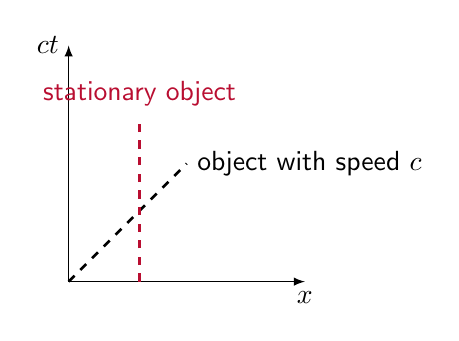
\begin{tikzpicture}
\tikzmath{
\L=3;
\xs=0.5*\L;
}
\draw[-latex] (0,0) -- (\L,0) node[below] {$x$};
\draw[-latex] (0,0) -- (0,\L) node[left] {$ct$};
\draw[dashed, line width=1] (0,0) -- (\L/2,\L/2) node[right] {object with speed $c$};
\draw[dashed, line width=1, color=qred] (0.3*\L,0) -- (0.3*\L,0.7*\L) node[above] {stationary object};
\end{tikzpicture}
\captionof*{figure}{\textit{Space-time diagram.}}
}

%%%%%%%%%%%%%%%%%%%%%%%%%%%%%%


%%%%%%%%%%%%%%%%%%%%%%%%%%%%%%
\subsection{Light cones}
\label{subsec:light cones}
\twocolframesf{Light cones}
{
\begin{itemize}
\item Since no signal can travel faster than the speed of light, there is always a limit as to where an object could have been in the past and where it could be in the future.
\item If an object is at the origin of a coordinate system at $t=0$, we can draw 2 cones that determine where the object could have been in the past and where it could be in the future.
\end{itemize}
}
{
\centering
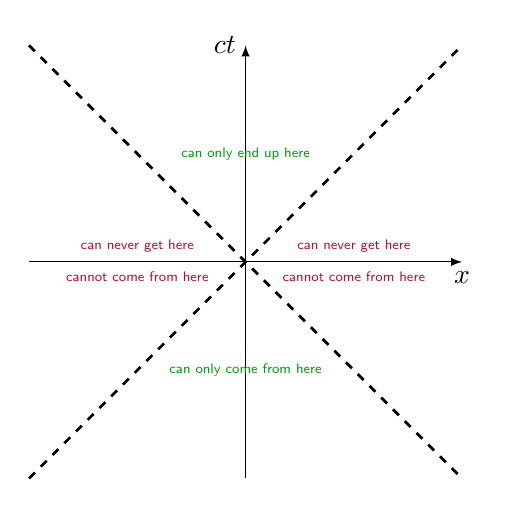
\begin{tikzpicture}
\tikzmath{
\L=2.75;
}
\draw[-latex] (-\L,0) -- (\L,0) node[below] {$x$};
\draw[-latex] (0,-\L) -- (0,\L) node[left] {$ct$};

\draw[dashed, line width=1] (-\L,-\L) -- (\L,\L);
\draw[dashed, line width=1] (-\L,\L) -- (\L,-\L);

\node[color=qred,above] at (\L/2,0) {\tiny can never get here};
\node[color=qred,below] at (\L/2,0) {\tiny cannot come from here};
\node[color=qred,above] at (-\L/2,0) {\tiny can never get here};
\node[color=qred,below] at (-\L/2,0) {\tiny cannot come from here};

\node[color=mygreen] at (0,\L/2) {\tiny can only end up here};
\node[color=mygreen] at (0,-\L/2) {\tiny can only come from here};

\end{tikzpicture}
\captionof*{figure}{\textit{Space-time diagram with light cones.}}
}

%%%%%%%%%%%%%%%%%%%%%%%%%%%%%%
\subsection{Space-time diagrams in different frames}
\label{subsec:spacetimediagramsindifferentframes}
\twocolframesf{Space-time diagrams in different frames}
{
\begin{itemize}
\item In space time, we can draw $S$ and $S’$ with the same origin.
\item However, because of the Lorentz transformation, the $(x,ct)$ axes of $S’$ are not perpendicular as viewed in $S$.
\item Suppose an event, $E_1$, occurs in space-time:
\begin{itemize}
\item<2-> In $S$, it has position ($x_1$,$ct_1$).
\item<3-> In $S’$, it has position ($x'_1$,$ct'_1$) given by Lorentz transformations.
\end{itemize}
\end{itemize}

}
{
\centering
\begin{tikzpicture}
\tikzmath{
\L=5;
\Eox=0.5*\L;
\Eoy=0.5*\L;
\th=20;
\v=1.*tan(\th);
\ga=1/sqrt(1-\v*\v);
\Eoxp=\ga*(\Eox-\v*\Eoy);
\Eoyp=\ga*(\Eoy-\v*\Eox);
}
\coordinate (E1) at (\Eox,\Eoy);
\coordinate (OO) at (0,0);
\coordinate (XP) at ($(0,0)+(\th:0.3*\L)$);
\coordinate (YP) at ($(0,0)+({90-\th}:0.3*\L)$);
\coordinate (E1YP) at ($(E1)+(\th:0.3*\L)$);
\coordinate (E1XP) at ($(E1)+({90-\th}:0.3*\L)$);
\coordinate (E1y) at (intersection of E1--E1YP and OO--YP);
\coordinate (E1x) at (intersection of E1--E1XP and OO--XP);


\draw[-latex] (0,0) -- (\L,0) node[below] {$x$};
\draw[-latex] (0,0) -- (0,\L) node[left] {$ct$};

\draw[-latex,color=qred] (0,0) -- (\th:\L) node[below] {$x'$};
\draw[-latex,color=qred] (0,0) -- ({90-\th}:\L) node[left] {$ct'$};

\only<1>{
\draw[color=qred] (0.2*\L,0) arc (0:\th:0.2*\L) node[midway,right]{$\tan\theta=\frac{v}{c}$};
}
\only<2->{
\draw[color=qred] (0.2*\L,0) arc (0:\th:0.2*\L) node[midway,right]{$\theta$};
}

\only<2->{
\fill (E1) circle(2pt);
\node[above] at (E1) {$E_1$};
\draw[dashed] (0,\Eoy) node[left]{$ct_1$} -- (E1) -- (\Eox,0)node[below]{$x_1$};	
}
\only<3->{
%\draw[dashed,color=qred]({90-\th}:\Eoxp)node[left]{$ct'_1$} -- (E1) -- (\th:\Eoyp)node[below]{$x'_1$};
\draw[dashed,color=qred] (E1y) node[left]{$ct'_1$} -- (E1) -- (E1x) node[below]{$x'_1$};
}
\end{tikzpicture}
\captionof*{figure}{\textit{Space-time diagram in two different reference frames}}
}

%%%%%%%%%%%%%%%%%%%%%%%%%%%%%%




%%%%%%%%%%%%%%%%%%%%%%%%%%%%%%
\subsection{Causality, space-like, time-like}
\label{subsec:causalityspaceliketimelike}
\twocolframesf{Causality, space like, time like}
{
\begin{itemize}
\item One event can only cause the other if it is in the past light cone: there is no reference frame where it could look like $E_2$ happened before $E_1$. These are called \textbf{“time like”}.
\item Two events that are outside each other’s light cones are called \textbf{“space like”} – they can never be causally connected. \emph{These are the only types of events where observers can disagree on the order}!
\end{itemize}
}
{
\centering
\begin{tikzpicture}
\tikzmath{
\L=2.75;
}
\draw[-latex] (-\L,0) -- (\L,0) node[below] {$x$};
\draw[-latex] (0,-\L) -- (0,\L) node[left] {$ct$};

\draw[dashed, line width=1] (-\L,-\L) -- (\L,\L);
\draw[dashed, line width=1] (-\L,\L) -- (\L,-\L);

\fill[color=qred] (0,0) circle(2pt);
\node[color=qred,right] at (0,0) {$E_2$};
\fill[color=qblue] (-0.2*\L,-0.5*\L) circle(2pt);
\node[color=qblue,right] at (-0.2*\L,-0.5*\L) {$E_1$};

\end{tikzpicture}
\captionof*{figure}{\textit{Space-time diagram showing time like events.}}
}



%%%%%%%%%%%%%%%%%%%%%%%%%%%%%%
%% Simultaneity Animation 1
%%%%%%%%%%%%%%%%%%%%%%%%%%%%%%
%%%%%%%%%%%%%%%%%%%%%%%%%%%%%%
\begin{frame}{Recall: Simultaneity}

\centering

\pgfmathtruncatemacro\N{24}
\begin{animateinline}[autoplay,loop]{4} % 5 fps, same as 0.2 s transduration

\multiframe{\N}{i=0+1}{

\tikzmath{
\L=10;
\w=0.2;%thickness of platform
\h=2;
\D=0.3*\L;
\x=0.33*\L-\i*\D/\N;
}
\begin{tikzpicture}
%\useasboundingbox (-0.7*\L,-3*\w) rectangle (0.7*\L,1.5*\h);
\useasboundingbox (-0.7*\L,-\h) rectangle (0.7*\L,1.5*\h);
%platform
\fill[color=black!70] (-\L/2,-\w) rectangle (\L/2,0);
%posts
\fill[color=qblue!70] (-0.42*\L,0) rectangle (-0.38*\L,0.97*\h);
\fill[color=qblue!70] (0.38*\L,0) rectangle (0.42*\L,0.97*\h);

%laser ball
\draw [color=qred, line width =1.5pt] (\x,1.2*\h) -- (0.35*\L,1.2*\h);
\draw [color=qred, line width =1.5pt] (-\x,1.2*\h) -- (-0.35*\L,1.2*\h);
\node [color=qred, star, star points=10, star point height=.1cm, minimum size=0.2cm, fill] at(\x,1.2*\h) {};
\node [color=qred, star, star points=10, star point height=.1cm, minimum size=0.2cm, fill] at(-\x,1.2*\h) {};


\ifthenelse{\i<23}{
\node[above=-0.2cm] at (0,0) {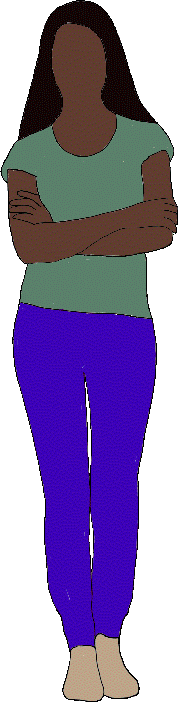
\includegraphics[width=0.04\textwidth]{figures/Relativity/woman_standing}};
}
{
\node[above=-0.5cm] at (-0.01*\L,0) {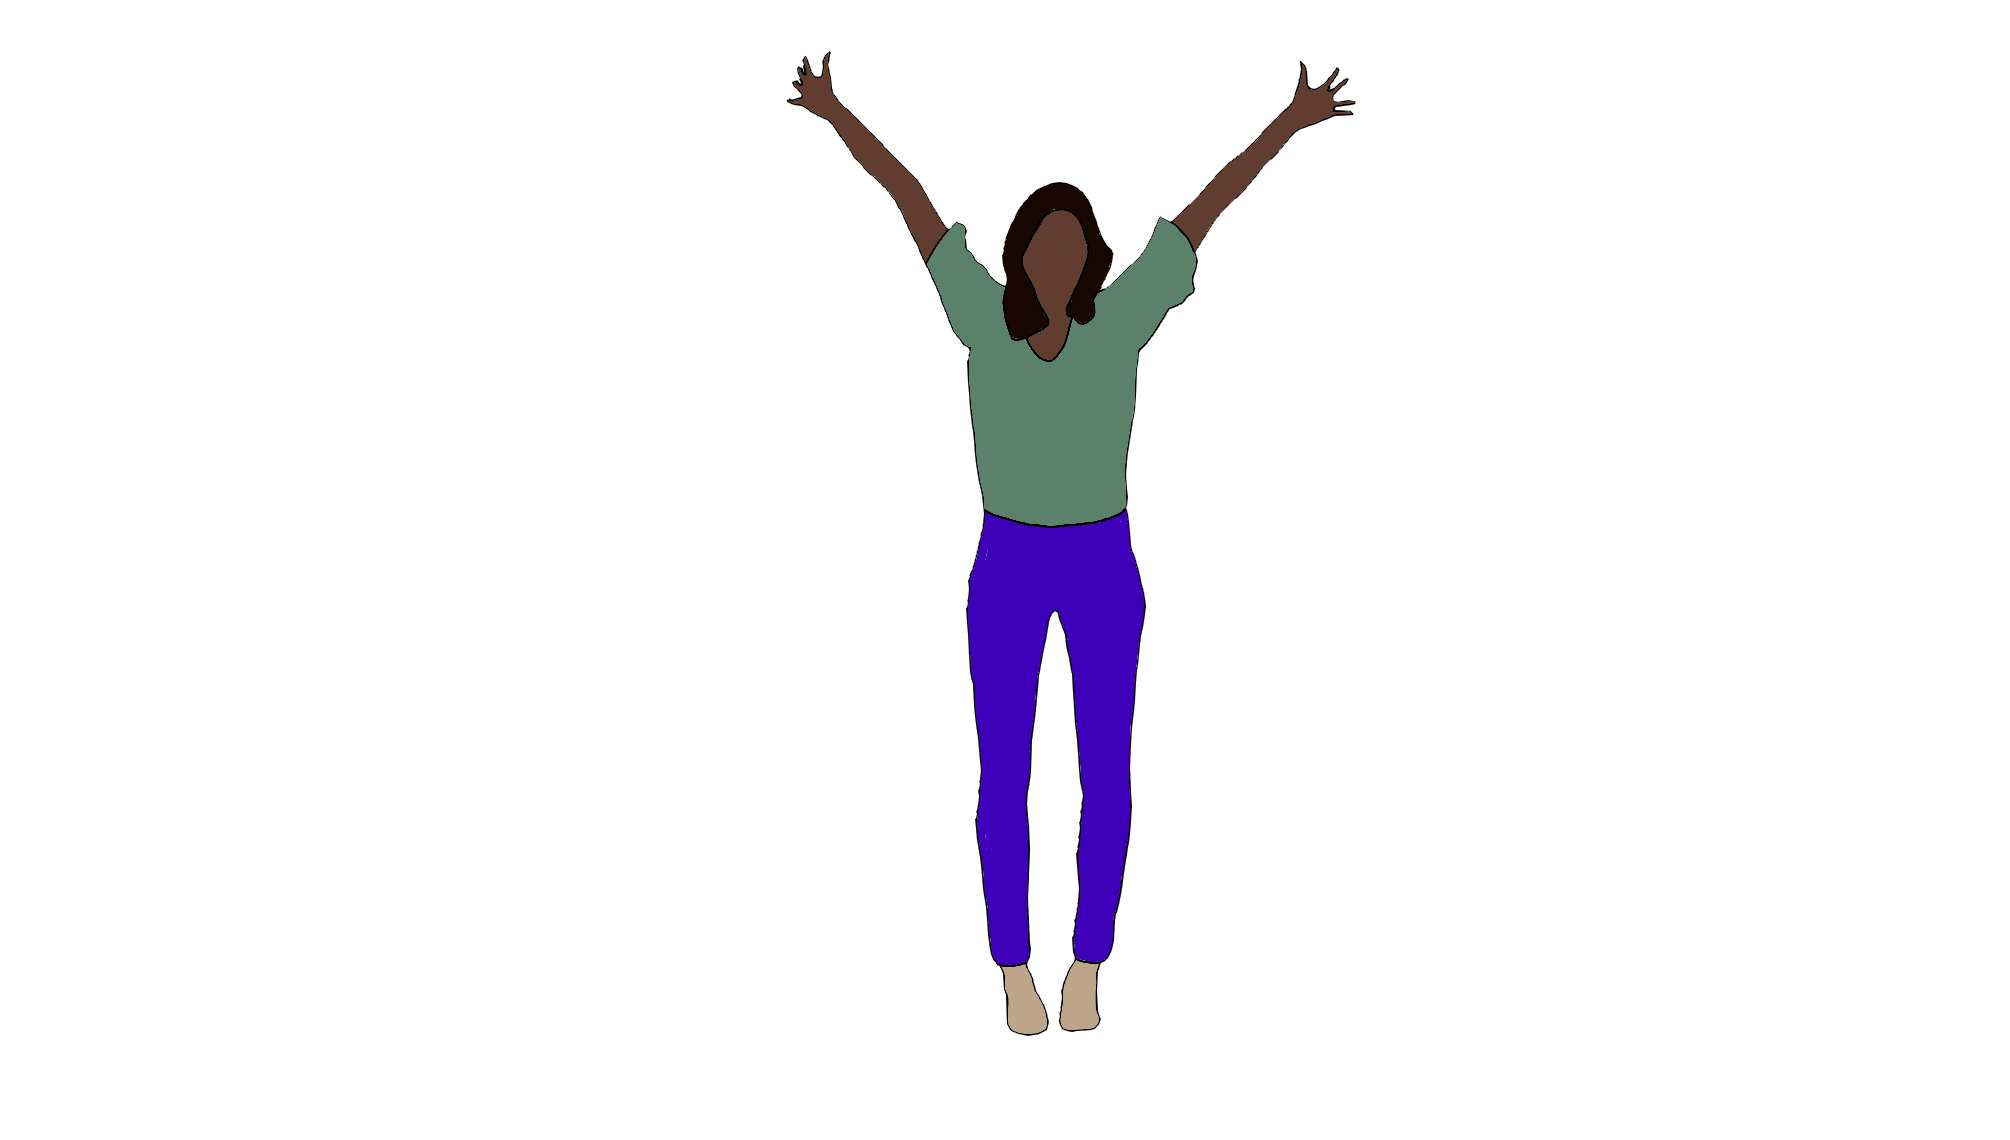
\includegraphics[width=0.4\textwidth]{figures/Relativity/alice_arms_png}};
}


\ifthenelse{\i<6}{
\node[above=-0.2cm] at (-0.4*\L,\h) {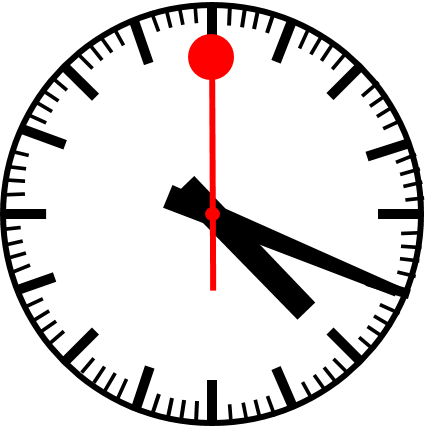
\includegraphics[width=0.07\textwidth]{figures/Relativity/fourtwenty.png}};
}{}
\ifthenelse{\i>5 \AND \i<12}{
\node[above=-0.2cm] at (-0.4*\L,\h) {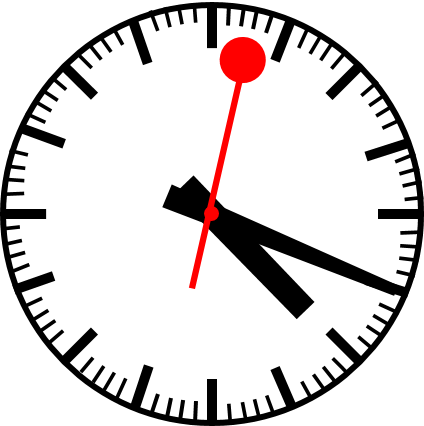
\includegraphics[width=0.07\textwidth]{figures/Relativity/fourtwenty_1.png}};
}{}
\ifthenelse{\i>11 \AND \i<18}{
\node[above=-0.2cm] at (-0.4*\L,\h) {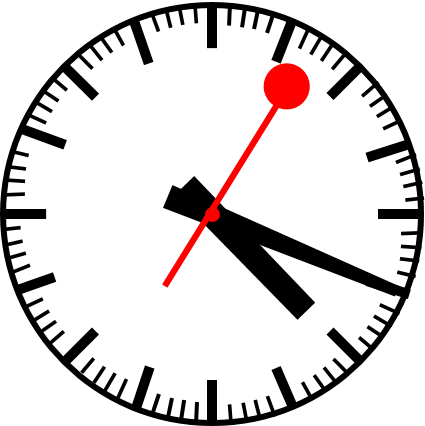
\includegraphics[width=0.07\textwidth]{figures/Relativity/fourtwenty_2.png}};
}{}
\ifthenelse{\i>17}{
\node[above=-0.2cm] at (-0.4*\L,\h) {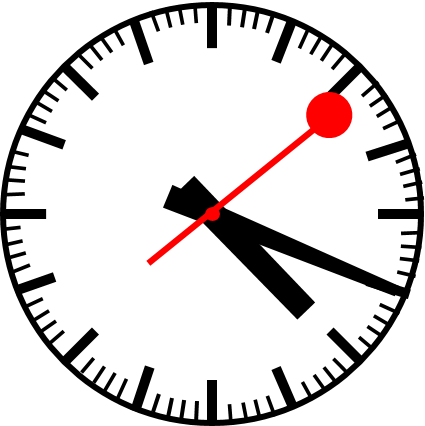
\includegraphics[width=0.07\textwidth]{figures/Relativity/fourtwenty_3.png}};
}{}

\ifthenelse{\i<6}{
\node[above=-0.2cm] at (0.4*\L,\h) {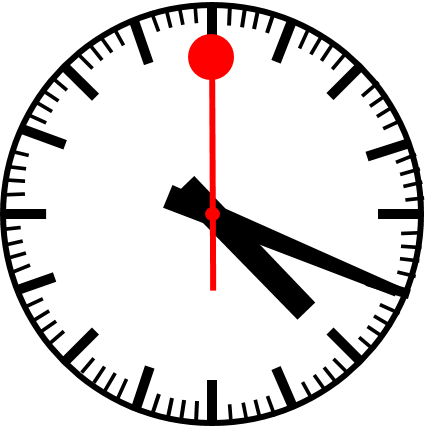
\includegraphics[width=0.07\textwidth]{figures/Relativity/fourtwenty.png}};
}{}
\ifthenelse{\i>5 \AND \i<12}{
\node[above=-0.2cm] at (0.4*\L,\h) {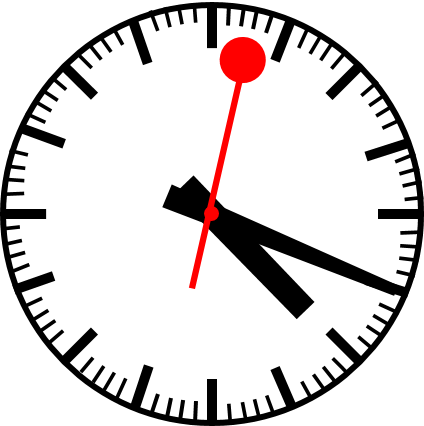
\includegraphics[width=0.07\textwidth]{figures/Relativity/fourtwenty_1.png}};
}{}
\ifthenelse{\i>11 \AND \i<18}{
\node[above=-0.2cm] at (0.4*\L,\h) {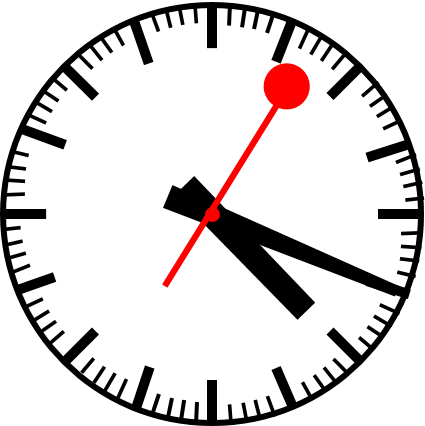
\includegraphics[width=0.07\textwidth]{figures/Relativity/fourtwenty_2.png}};
}{}
\ifthenelse{\i>17}{
\node[above=-0.2cm] at (0.4*\L,\h) {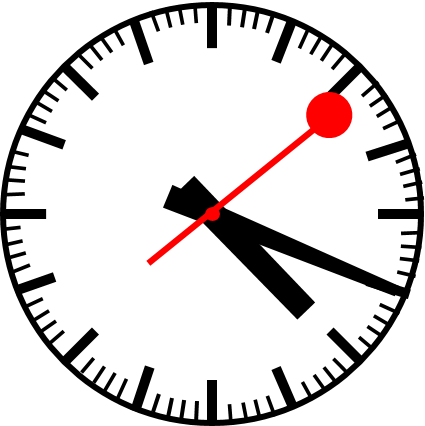
\includegraphics[width=0.07\textwidth]{figures/Relativity/fourtwenty_3.png}};
}{}

\end{tikzpicture}
}%multiframe
\end{animateinline}


\begin{itemize}
\item An observer on a platform is equidistant from 2 clocks that output pulses of light. When the clocks read 16:20, they output a light pulse, the observer sees the two light pulses at the same time and she concludes that the clock are synchronized.
\end{itemize}

\end{frame}


%%%%%%%%%%%%%%%%%%%%%%%%%%%%%%
%% Simultaneity Animation 2
%%%%%%%%%%%%%%%%%%%%%%%%%%%%%%
%%%%%%%%%%%%%%%%%%%%%%%%%%%%%%
\begin{frame}{Recall: Simultaneity}

\centering

\pgfmathtruncatemacro\N{24}
\begin{animateinline}[autoplay,loop]{4} % 5 fps, same as 0.2 s transduration

\multiframe{\N}{i=0+1}{

\tikzmath{
%\i=1;
\L=10;
\w=0.2;%thickness of platform
\h=2;
\D=0.3*\L;
\xs=0.25*\L-\i*0.5*\L/\N;%platform shift
\xr=\xs+0.33*\L-\i*\D/\N;%position of right laser
\xl=-\xs+0.33*\L+\i*\D/\N-1.12*\L;%position of left laser
}
\begin{tikzpicture}

\useasboundingbox (-0.7*\L,-\h) rectangle (0.7*\L,1.5*\h);


%moving platform
\begin{scope}[shift={(\xs,0)}]
%platform
\fill[color=black!70] (-\L/2,-\w) rectangle (\L/2,0);
%posts
\fill[color=qblue!70] (-0.42*\L,0) rectangle (-0.38*\L,0.97*\h);
\fill[color=qblue!70] (0.38*\L,0) rectangle (0.42*\L,0.97*\h);
\ifthenelse{\i<23}{
\node[above=-0.2cm] at (0,0) {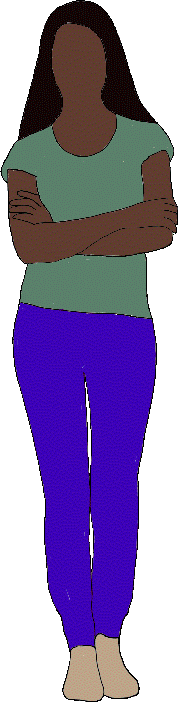
\includegraphics[width=0.04\textwidth]{figures/Relativity/woman_standing}};
}
{
\node[above=-0.5cm] at (-0.01*\L,0) {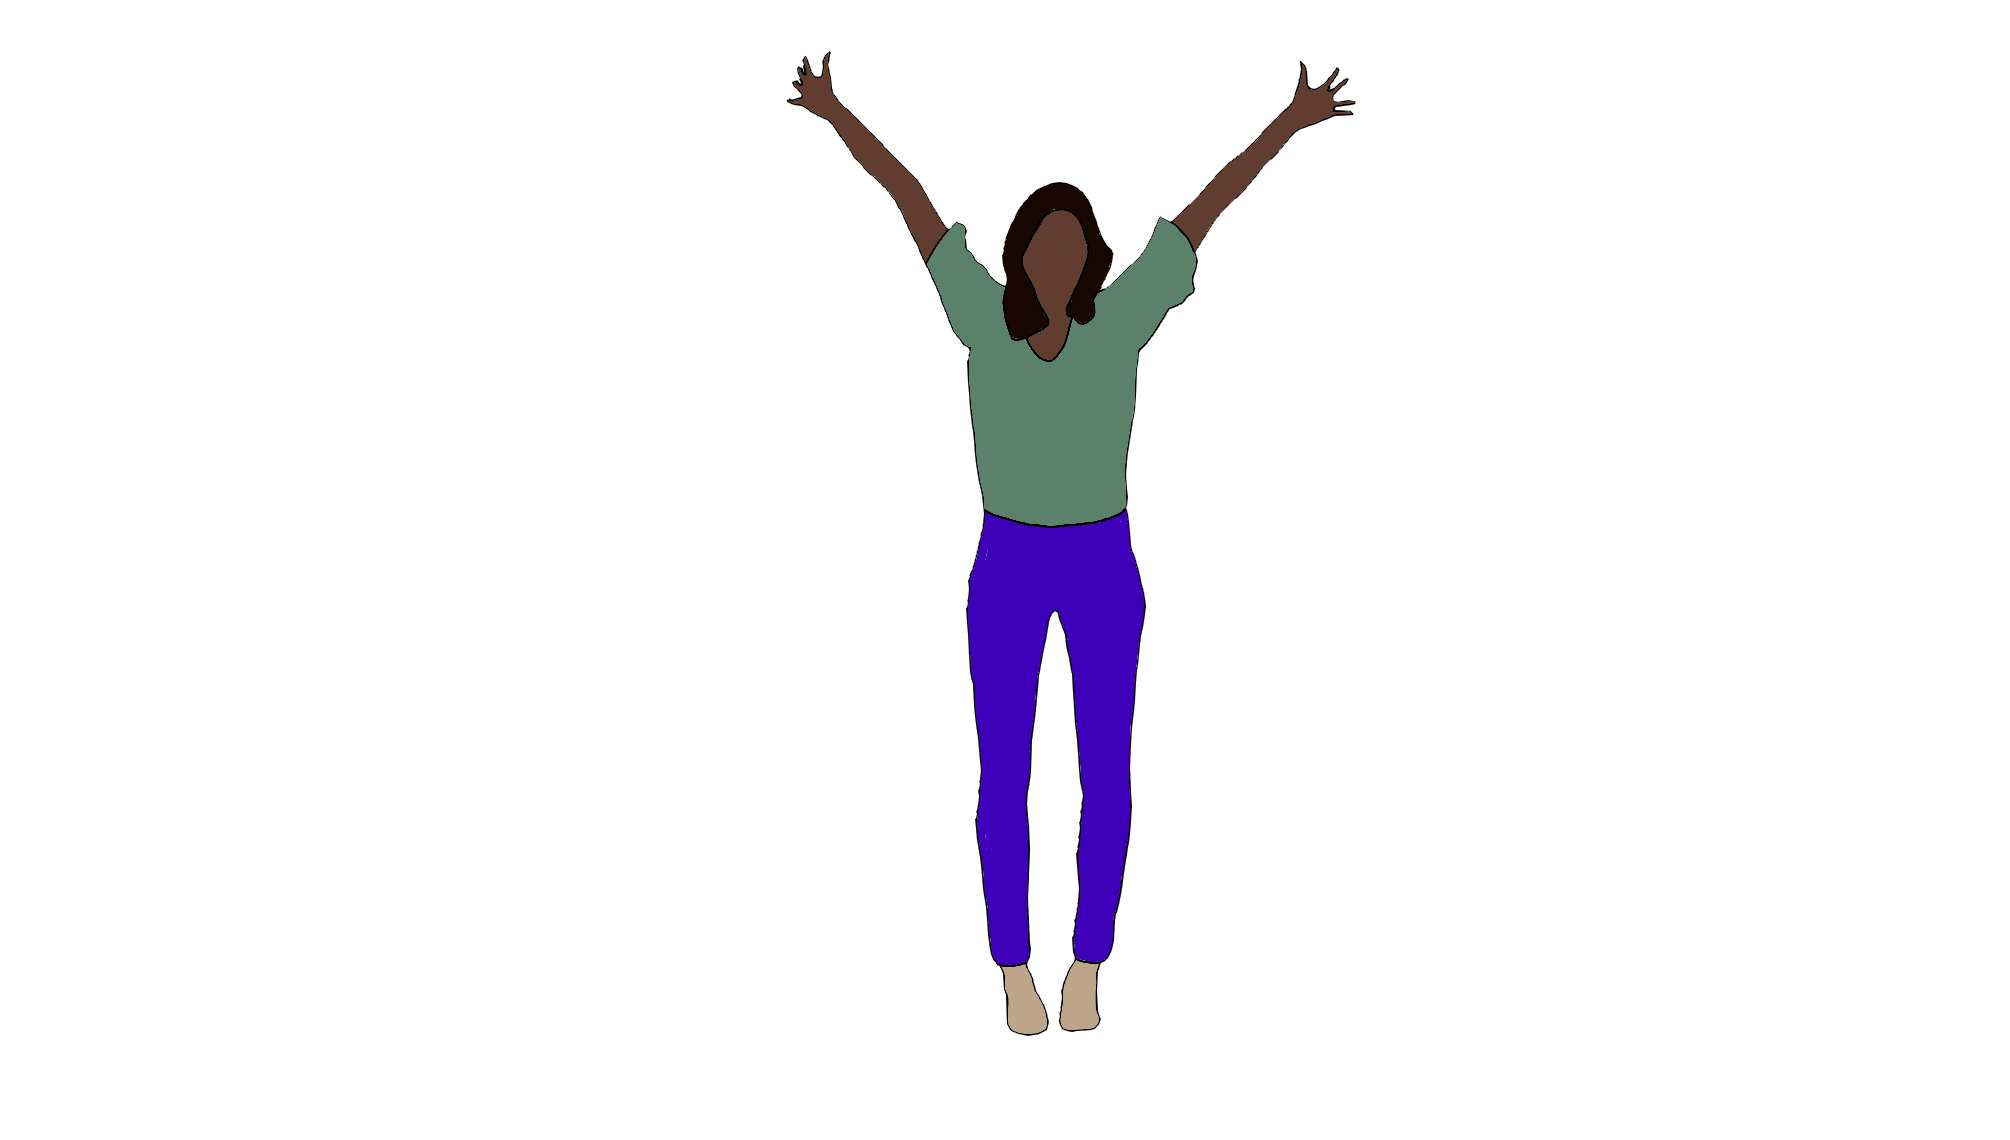
\includegraphics[width=0.4\textwidth]{figures/Relativity/alice_arms_png}};
}

%left clock
\ifthenelse{\i<5}{
\node[above=-0.2cm] at (-0.4*\L,\h) {
\includegraphics[width=0.07\textwidth]{figures/Relativity/fourtwenty_m3.png}};
}{}
\ifthenelse{\i>4 \AND \i<11}{
\node[above=-0.2cm] at (-0.4*\L,\h) {
\includegraphics[width=0.07\textwidth]{figures/Relativity/fourtwenty_m2.png}};
}{}
\ifthenelse{\i>10 \AND \i<17}{
\node[above=-0.2cm] at (-0.4*\L,\h) {
\includegraphics[width=0.07\textwidth]{figures/Relativity/fourtwenty_m1.png}};
}{}
\ifthenelse{\i>16}{
\node[above=-0.2cm] at (-0.4*\L,\h) {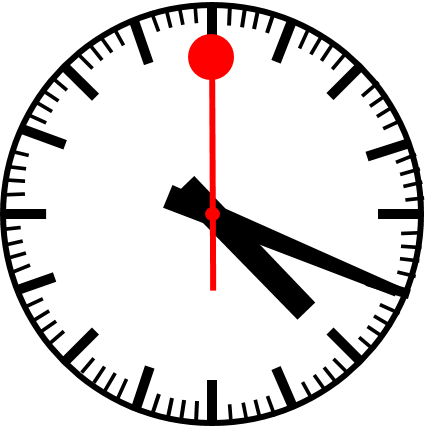
\includegraphics[width=0.07\textwidth]{figures/Relativity/fourtwenty.png}};
}{}


%right clock
\ifthenelse{\i<5}{
\node[above=-0.2cm] at (0.4*\L,\h) {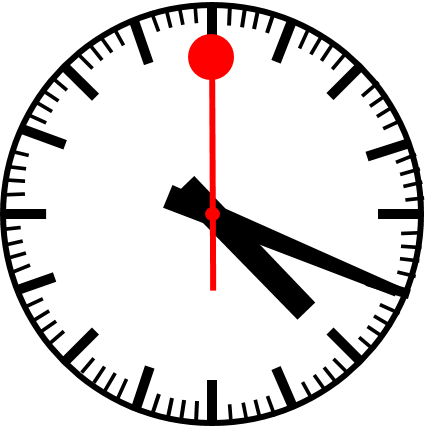
\includegraphics[width=0.07\textwidth]{figures/Relativity/fourtwenty.png}};
}{}
\ifthenelse{\i>4 \AND \i<11}{
\node[above=-0.2cm] at (0.4*\L,\h) {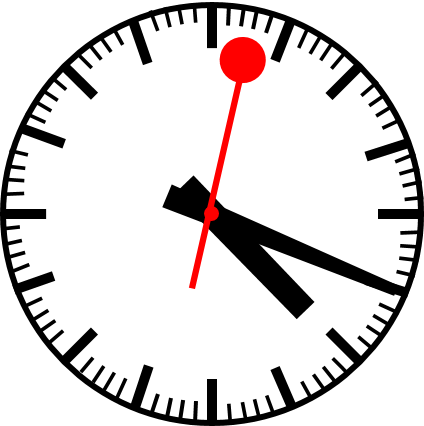
\includegraphics[width=0.07\textwidth]{figures/Relativity/fourtwenty_1.png}};
}{}
\ifthenelse{\i>10 \AND \i<17}{
\node[above=-0.2cm] at (0.4*\L,\h) {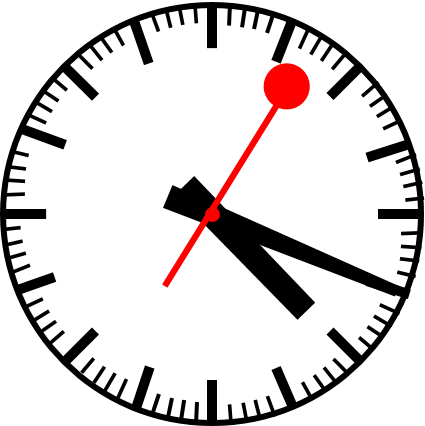
\includegraphics[width=0.07\textwidth]{figures/Relativity/fourtwenty_2.png}};
}{}
\ifthenelse{\i>16}{
\node[above=-0.2cm] at (0.4*\L,\h) {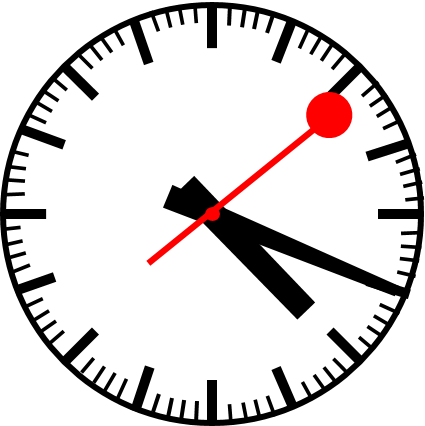
\includegraphics[width=0.07\textwidth]{figures/Relativity/fourtwenty_3.png}};
}{}

\end{scope}

%foreground person
\node[above=-0.5cm] at (-0.5*\L,-0.5*\h) {
\includegraphics[width=0.4\textwidth]{figures/Relativity/traincart}};
\node[above=0cm] at (-0.5*\L,-0.5*\h) {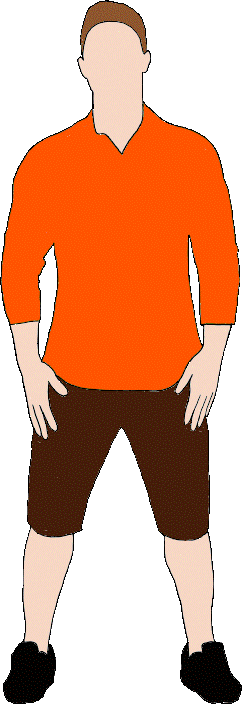
\includegraphics[width=0.06\textwidth]{figures/Relativity/man_standing_ink}};


%laser ball
\draw [color=qred, line width =1.5pt] (\xr,1.2*\h) -- (0.6*\L,1.2*\h);
\node [color=qred, star, star points=10, star point height=.1cm, minimum size=0.2cm, fill] at(\xr,1.2*\h) {};
\ifthenelse{\i>16}{
\draw [color=qred, line width =1.5pt] (\xl,1.2*\h) -- (-0.5*\L,1.2*\h);
\node [color=qred, star, star points=10, star point height=.1cm, minimum size=0.2cm, fill] at(\xl,1.2*\h) {};
}{}

\end{tikzpicture}
}%multiframe
\end{animateinline}

\begin{itemize}
\item An observer on a train sees the platform moving in his rest frame. He observes two pulses of light arrive at the same time at the person on the platform. 
\item He concludes that the pulse from the right happened first, since the pulses travel at speed $c$ and the one from the right traveled further. He disagrees that the clocks are synchronized!
\end{itemize}

\end{frame}




%%%%%%%%%%%%%%%%%%%%%%%%%%%%%%
\subsection{Space-time diagram for platform clocks}
\label{subsec:spcaetimediagramforplatformclocks}
\begin{frame}{Space-time diagram for platform clocks}
Draw the space time diagram for the case of the person on the platform in the middle of the two clocks:
\begin{itemize}
\item Event A: Clock A emits a pulse of light
\item Event B: Clock B emits a pulse of light
\item Event C: The pulses of light meet at the position of the person
\end{itemize}
After drawing this in frame $S$ (the platform), draw $S’$ on top of that (the frame for the moving train), and compare the locations of $A$ and $B$…
\capfig{0.5}{figures/Relativity/platform}{In the reference frame at rest relative to the clocks, they appear synchronized, emitting pulses of light at the same time.}
\end{frame}



%%%%%%%%%%%%%%%%%%%%%%%%%%%%%%
\twocolframe{Space-time diagram for platform clocks}
{
\only<1>{
\capfig{0.9}{figures/Relativity/platform_rest}{In the reference frame at rest relative to the clocks.}
}
\only<2>{
\capfig{0.9}{figures/Relativity/platform_moving}{In the reference frame moving relative to the clocks.}
}
\only<3>{
\scalebox{-1}[1]{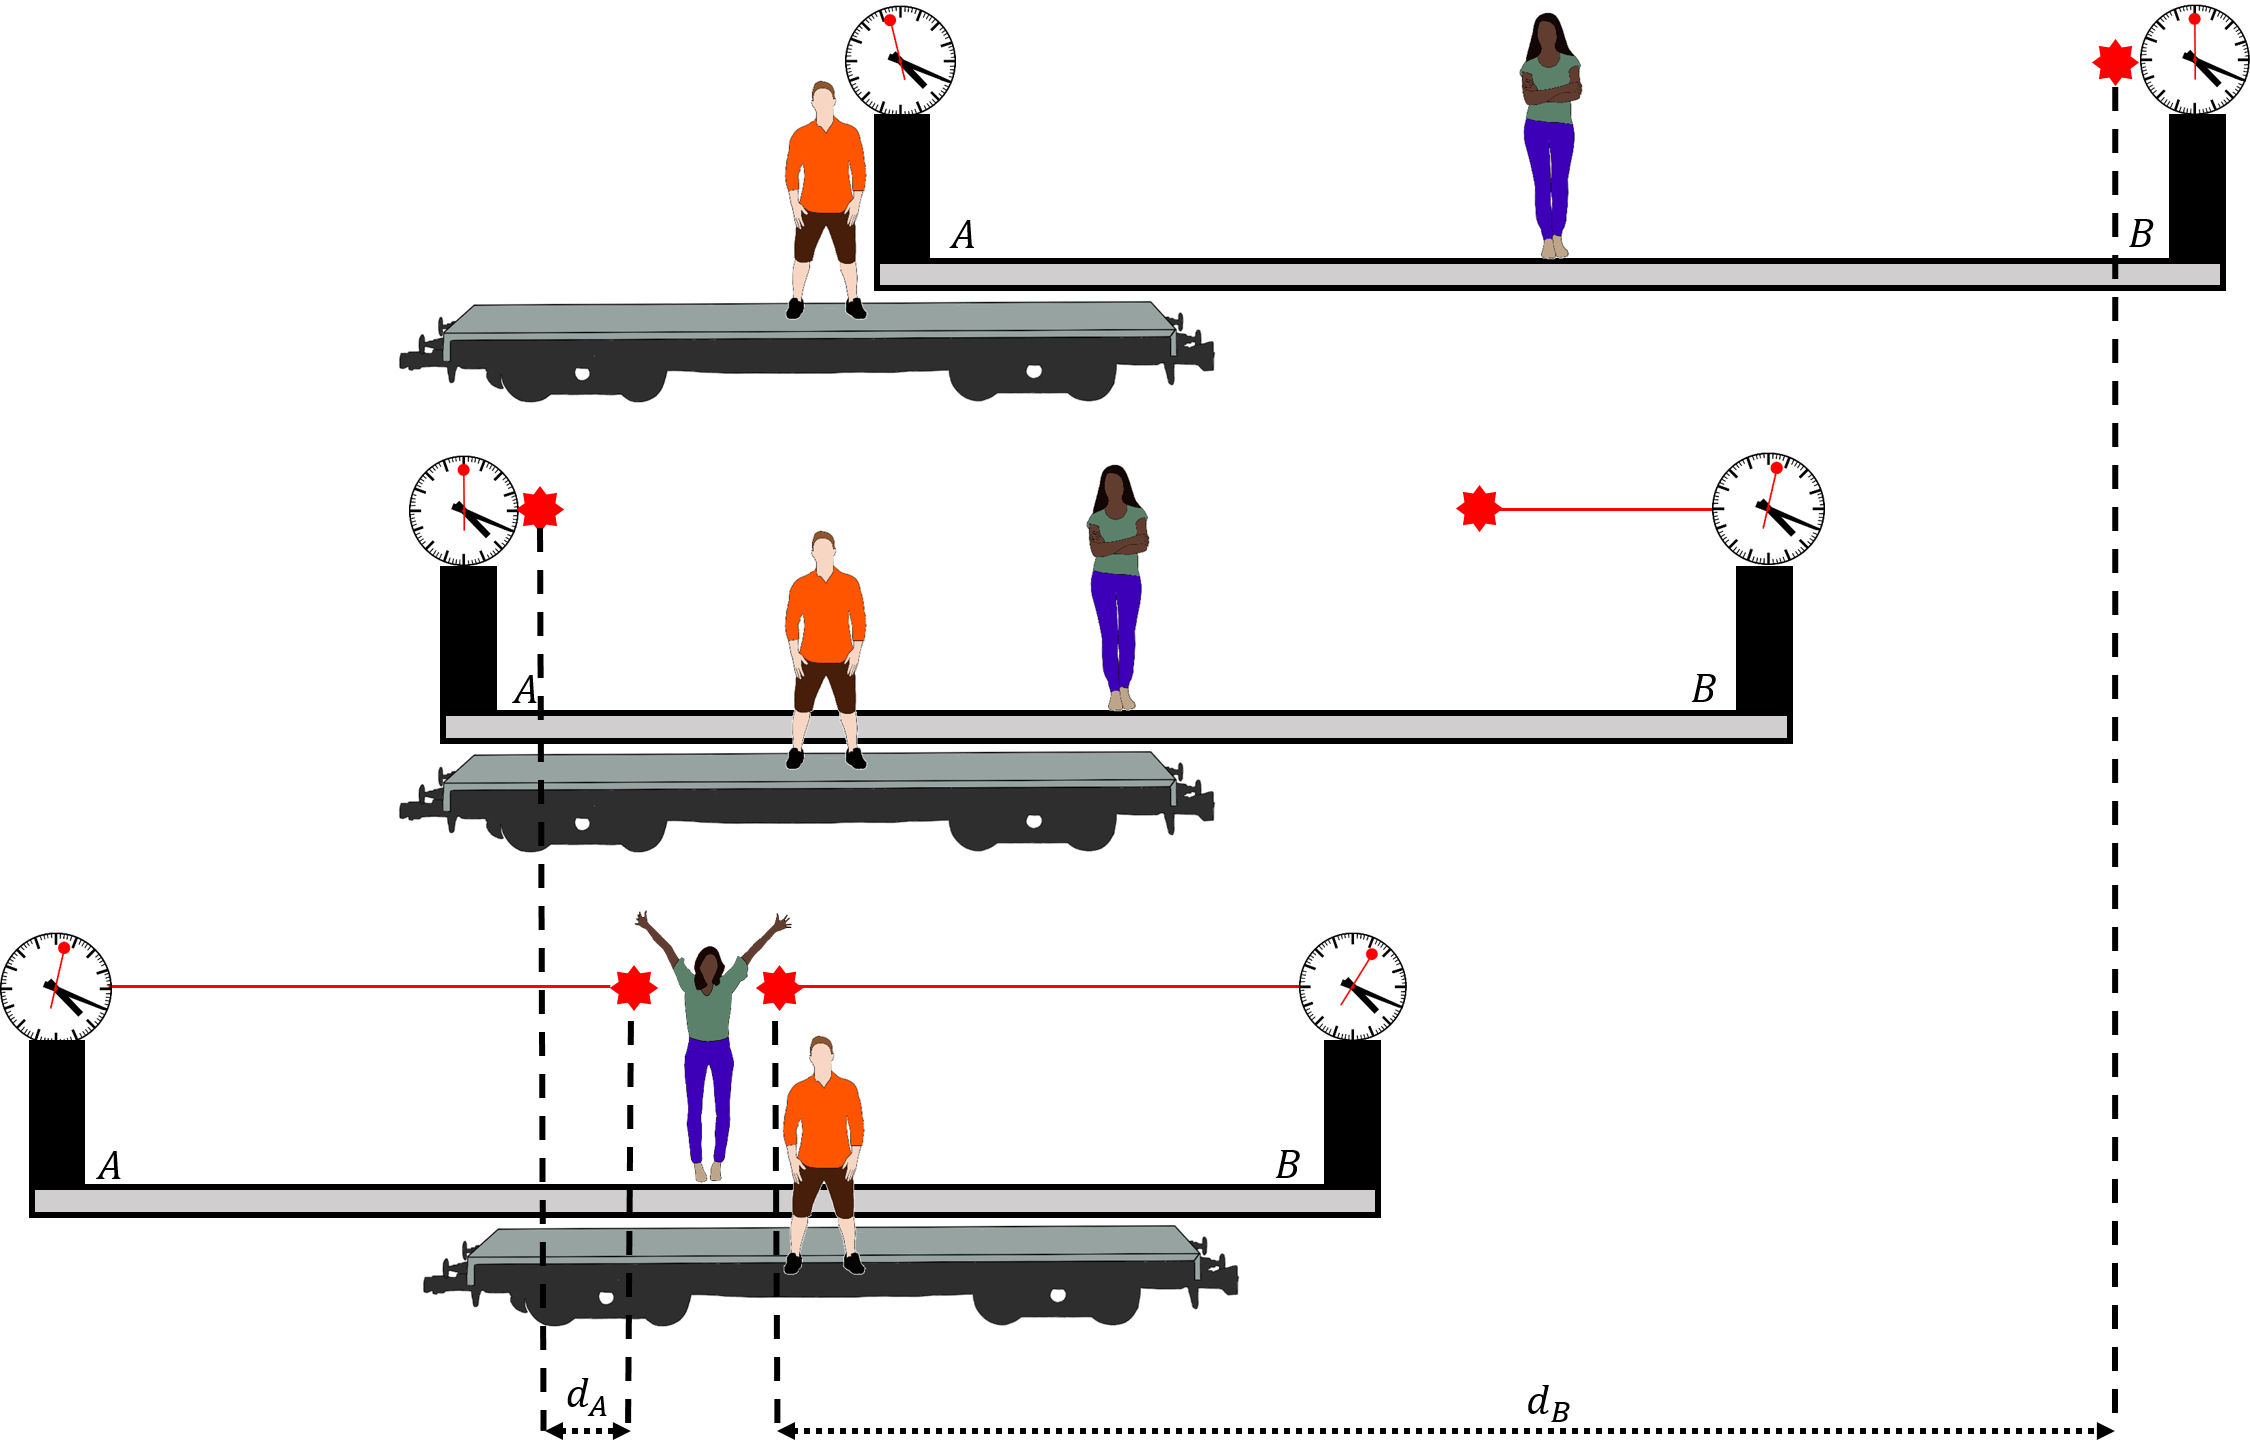
\includegraphics[width=0.9\textwidth]{figures/Relativity/platform_moving}}
\captionof*{figure}{\textit{In the reference frame moving relative to the clocks, going the other way.}}
}
}
{
\centering
\begin{tikzpicture}
\tikzmath{
\L=4.5;
\EAx=-0.3*\L;
\EAy=0.*\L;
\EBx=0.3*\L;
\EBy=0.*\L;
\ECx=0;
\ECy=\EBx;
\th=20;
\v=1.*tan(\th);
}
\coordinate (EA) at (\EAx,\EAy);
\coordinate (EB) at (\EBx,\EBy);
\coordinate (EC) at (\ECx,\ECy);
\coordinate (OO) at (0,0);

\draw[-latex,line width = 1] (-0.5*\L,0) -- (0.75*\L,0) node[below] {$x$};
\draw[-latex,line width = 1] (0,-0.5*\L) -- (0,0.75*\L) node[left] {$ct$};

\fill (EA) circle(2pt) node[above]{$A$};
\fill (EB) circle(2pt) node[above]{$B$};
\fill (EC) circle(2pt) node[left]{$C$};

\draw[color=qred,line width = 1] (EA) -- (EC);
\draw[color=qred,line width = 1] (EB) -- (EC);

%S' axes
\only<3>{
\tikzmath{\th=-20;}
}

\only<2->{
\draw[-latex,color=qblue!70,line width = 1] (\th:-0.5*\L) -- (\th:0.75*\L) node[below] {$x'$};
\draw[-latex,color=qblue!70,line width = 1] ({90-\th}:-0.5*\L) -- ({90-\th}:0.75*\L) node[left] {$ct'$};

\coordinate (XP) at ($(0,0)+(\th:0.3*\L)$);
\coordinate (YP) at ($(0,0)+({90-\th}:0.3*\L)$);
\coordinate (EAYP) at ($(EA)+(\th:0.3*\L)$);
\coordinate (EAy) at (intersection of EA--EAYP and OO--YP);
\coordinate (EBYP) at ($(EB)+(\th:0.3*\L)$);
\coordinate (EBy) at (intersection of EB--EBYP and OO--YP);
\coordinate (ECYP) at ($(EC)+(\th:0.3*\L)$);
\coordinate (ECy) at (intersection of EC--ECYP and OO--YP);

\draw[dashed,color=qblue!70] (EA) -- (EAy);
\fill[color=qblue!70] (EAy) circle(2pt);
\draw[dashed,color=qblue!70] (EB) -- (EBy);
\fill[color=qblue!70] (EBy) circle(2pt);
\draw[dashed,color=qblue!70] (EC) -- (ECy);
\fill[color=qblue!70] (ECy) circle(2pt);
}
\end{tikzpicture}
\captionof*{figure}{\textit{Space-time diagram for platform clocks}}
}


%%%%%%%%%%%%%%%%%%%%%%%%%%%%%%
\begin{frame}{The Train Paradox}
\capfig{1}{figures/Relativity/barn}{}
\vspace{-1cm}
\begin{itemize}
\item As seen from the ground, the train that is contracted to a length of \SI{200}{m} fits in the tunnel of the same length. As seen in the train, the \SI{500}{m} train does not fit in the \SI{80}{m} tunnel. 
\item A person on Earth briefly closes the doors of the tunnel while the train is inside, nothing happens to the train, since it fits. To the observer on the train, was the train just destroyed?
\end{itemize}
\end{frame}

%%%%%%%%%%%%%%%%%%%%%%%%%%%%%%


%%%%%%%%%%%%%%%





%%%%%%%%%%%%%%%%






%%%%%%%%%%%%%%%%





\end{document}



